\documentclass{report}
\usepackage{amsmath}
\usepackage{ngerman}
\usepackage[hidelinks]{hyperref}
\usepackage[numbered]{bookmark}
\usepackage{pgfplots}
\usepackage{amssymb}

\usepgfplotslibrary{fillbetween}
\pgfplotsset{compat=1.18}
\tracinglostchars=2

\title{\textbf{Mathe-Abitur}}
\author{Tim Teichmann}
\date{\today}

\begin{document}
\maketitle
\tableofcontents

\chapter{Analysis}

\section{Funktionsscharen}
\subsection{Definition}
\begin{flushleft}
    Eine Funktionsschar ist eine Funktion, die auch von anderen Parametern als $x$ abhängt.
    Durch einen weiteren Parameter kann es plötzlich unendlich viele Variationen von der ursprünglichen Funktion geben.
    Das ist auch der Grund dafür, dass solch eine Funktion, Funktionsschar genannt wird.
    Es entsteht eine Menge -- also ein Schar -- von Funktionen.
\end{flushleft}

\subsection{Beispiel}
\begin{flushleft}
    Das ist beispielsweise eine quadratische Funktionsschar, die von den Parametern $x$ und $k$ abhängt.
    \begin{align}
        f_k(x)=kx^2
    \end{align}
    Der Parameter $k$ bestimmt nur die Stauchung der Funktion.
\end{flushleft}

\begin{center}
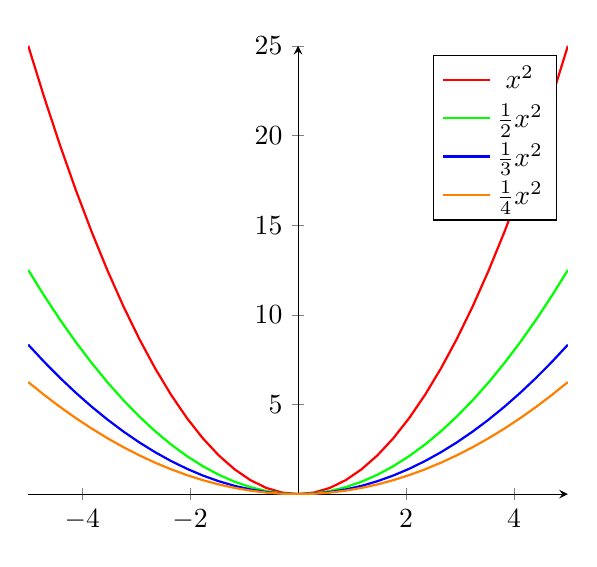
\begin{tikzpicture}
\begin{axis}[
    axis lines=middle,
    samples=35,
    domain=-5:5,
    every axis plot/.append style={thick},
]
\addplot[
    color=red,
]
{x^2};
\addlegendentry{$x^2$}

\addplot[
    color=green,
]
{0.5*x^2};
\addlegendentry{$\frac{1}{2}x^2$}

\addplot[
    color=blue,
]
{0.3333*x^2};
\addlegendentry{$\frac{1}{3}x^2$}

\addplot[
    color=orange,
]
{0.25*x^2};
\addlegendentry{$\frac{1}{4}x^2$}

\end{axis}
\end{tikzpicture}
\end{center}

\section{Trassierungsaufgaben}
\subsection{Definition}
\begin{flushleft}
    Das Ziel von Trassierungsaufgaben ist es anhand von bestimmten Angaben eine Funktion aufzustellen.
    Deshalb ist das Verstehen der Aufgabenstellung der schwierigste Teil der Aufgabe.
\end{flushleft}

\subsection{Beispiel}
\begin{flushleft}
    Das ist eine mögliche Aufgabenstellung: \\
    \textit{Eine quadratische Funktion hat im Punkt $P(0|0)$ eine Nullstelle und im Punkt $Q(2|5)$ ein Maximum. Stelle die Funktionsgleichung auf!} \\
    \begin{enumerate}
        \item {
                Die ersten drei Wörter des Satzes: \textbf{\textit{Eine quadratische Funktion}} sagen uns um welchen Typ Funktion es sich handelt.
                Es ist eine quadratische Funktion. Die allgemeine quadratische Funktion sieht so aus:
                \begin{align}
                    f(x)=ax^2+bx+c
                \end{align}
                Unsere Funktion $f$ hat also drei unbekannte, $a$, $b$ und $c$.
            }
        \item {
                Außerdem ist für uns wichtig, dass die Funktion \textbf{\textit{im Punkt $P(0|0)$ eine Nullstelle}} hat.
                Das bedeutet, dass $f(0)=0$ sein muss.
                Unsere erste Bedingung ist also:
                \begin{align}
                    f(0)=0
                \end{align}
            }
        \item {
                Als letztes hat unsere Funktion \textbf{\textit{im Punkt $Q(2|5)$ ein Maximum}}. \\
                Um die Extrempunkte von einer Funktion (hier: $g$) zu finden, muss man die erste Ableitung dieser Funktion gleich $0$ setzen.
                \begin{align}
                    g'(x)=0
                \end{align}
                Im Idealfall bekommt man eine oder mehr Lösungen heraus, wir nennen die Lösung $x_1$.
                Um herauszufinden um welche Art von Extrempunkt es sich handelt setzen wir $x_1$ in die zweite Ableitung von $g$ ein.
                \begin{align}            
                    g''(x) =
                    \begin{cases}
                        \text{Maximum}, &\text{wenn } x < 0 \\
                        \text{Minimum}, &\text{wenn } x > 0
                    \end{cases}
                \end{align}
                Jetzt können wir drei weitere Bedingungen für unsere Aufgabe aufstellen.
                Unsere Funktion soll ein Maximum in $Q(2|5)$ haben, deshalb müssen diese Bedingungen erfüllt sein:
                \begin{align}
                    f(2)=5 \\
                    f'(2)=0 \\
                    f''(2) < 0
                \end{align}
            }
        \item {
                Jetzt müssen wir aus unseren vier Bedingungen eine Funktion bilden, dafür bilden wir erstmal die ersten beiden Ableitungen.
                \begin{align}
                    f(x)&=ax^2+bx+c \\
                    f'(x)&=2ax+b \\
                    f''(x)&=2a \\
                    f(0)&=0 \\
                    f(2)&=5 \\
                    f'(2)&=0 \\
                    f''(2) & < 0
                \end{align}
                Nun müssen wir einsetzen, Ungleichungen ($f''(2) < 0$) dürfen nicht eingesetzt werden.
                \begin{align}
                    0^2a+0b+c &=0 \\
                    c &=0 \\
                    a*2^2+2b+c &= 5 \\
                    4a+2b+c &= 5 \\
                    4a+2b &= 5 \\
                    2a*2+b &=0 \\
                    4a+b &= 0
                \end{align}
                Eine von den drei unbekannten ist gelöst ($c=0$).
                Jetzt muss $4a+2b=5$ in $4a+b=0$ eingesetzt werden.
                \begin{align}
                    4a+2b &=5 \\
                    4a+b &= 0 \\
                    4a+2b-(4a+b) &= 5 \\
                    b &= 5 \\
                    4a+5 &= 0 \\
                    a &= \frac{-5}{4}
                \end{align}
                Alle unbekannten Variablen sind gelöst, $a=\frac{-5}{4}$, $b=5$, $c=0$.
                Also ist das unsere Funktion:
                \begin{align}
                    f(x)=\frac{-5}{4}x^2+5x
                \end{align}
            }
    \end{enumerate}
\end{flushleft}

\begin{center}
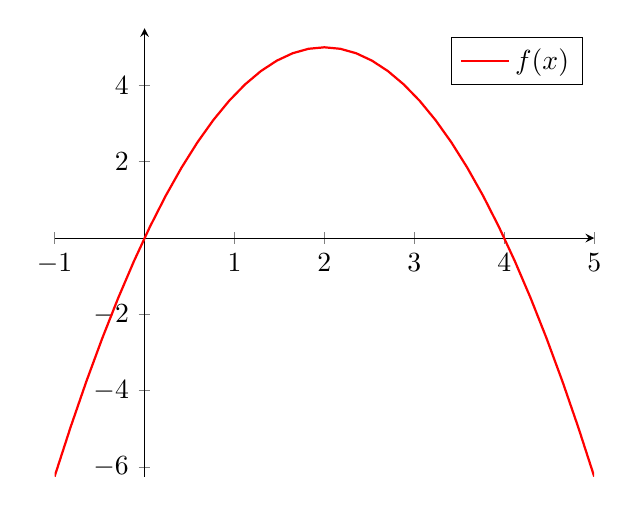
\begin{tikzpicture}
\begin{axis}[
    axis lines=middle,
    samples=35,
    domain=-1:5,
    ymax=5.5,
    every axis plot/.append style={thick},
]
\addplot[
    color=red,
]
{(-5/4)*((\x)*(\x))+(5)*(\x)};
\addlegendentry{$f(x)$}

\end{axis}
\end{tikzpicture}
\end{center}

\section{Extremwertaufgaben}
\subsection{Definition}
\begin{flushleft}   
    Bei Extemwertaufgaben geht es darum die maximal/minimal möglichen Flächeninhalte herauszufinden.
    Dabei kann es oft auch um das maximale/minimale Volumen eines Körpers gehen.
    Jedoch maximiert/minimiert sich das Volumen eines Körpers wenn der Flächeninhalt des Mantels maximal/minimal wird.
    Die Aufgabenstellungen zu diesem Aufgabentyp sind meistens sehr spezifisch und brauchen eine Skizze.
\end{flushleft}

\subsection{Beispiel}
\begin{flushleft}
    In diesem Beispiel soll der maximale Flächeninhalt eines Dreiecks gefunden werden.
    Das Dreieck ist unterhalb der Funktion $f$.
    Die drei Ecken des Dreiecks sind die Punkte $P(u|v)$, $Q(0|0)$ und $R(u|0)$.
    \begin{align}
        f(x)=x^3-6x^2+9x
    \end{align}
\end{flushleft}

\begin{center}
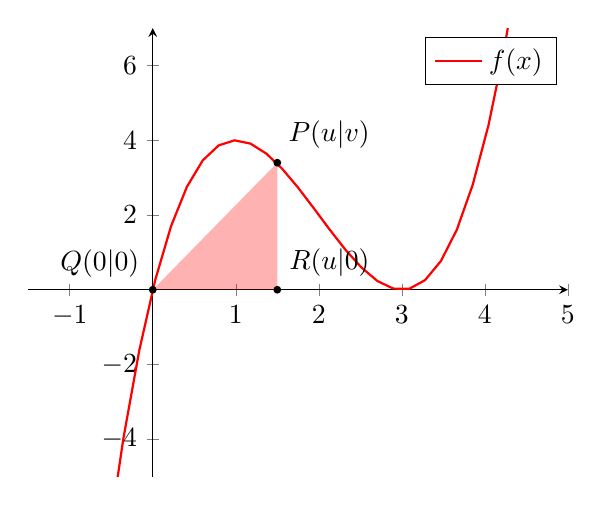
\begin{tikzpicture}   
\begin{axis}[
    axis lines=middle,
    samples=35,
    domain=-1.5:5,
    ymax=7,
    ymin=-5,
    every axis plot/.append style={thick},
]
\addplot[
    color=red,
    name path=A
]
{((\x)*(\x)*(\x))-(6*(\x)*(\x))+(9*(\x))};
\addlegendentry{$f(x)$}

\addplot[draw=none,name path=B] {(3.4/1.5)*(\x)};
\addplot[draw=none,name path=C] {0};
\addplot[red,opacity=0.3] fill between[of=B and C,soft clip={domain=0:1.5}];

\node[label={150:{$Q(0|0)$}},circle,fill,inner sep=1pt] at (axis cs:0,0) {};
\node[label={70:{$P(u|v)$}},circle,fill,inner sep=1pt] at (axis cs:1.5,3.4) {};
\node[label={60:{$R(u|0)$}},circle,fill,inner sep=1pt] at (axis cs:1.5,0) {};

\end{axis}
\end{tikzpicture}
\end{center}

\begin{flushleft}
    Um die Fläche $A$ eines Dreiecks auszurechnen nutzt man diese Formel, $g$ steht für die Grundseite und $h$ für die Höhe:
    \begin{align}
        A=\frac{gh}{2}
    \end{align}
    Mit $g$ und $h$ sieht der Plot so aus:
\end{flushleft}

\begin{center}
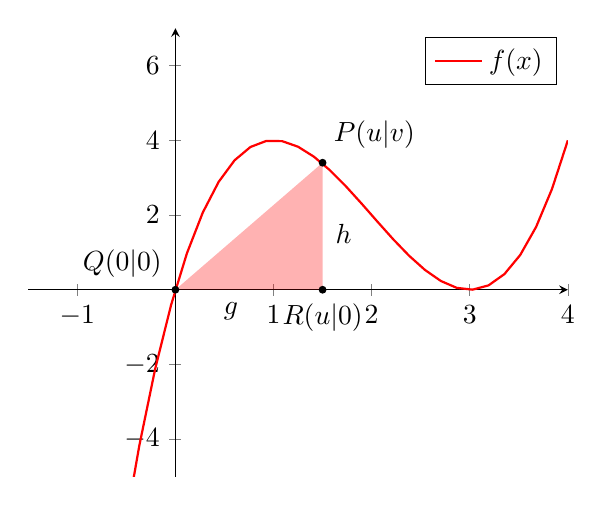
\begin{tikzpicture}   
\begin{axis}[
    axis lines=middle,
    samples=35,
    domain=-1.5:4,
    ymax=7,
    ymin=-5,
    every axis plot/.append style={thick},
]
\addplot[
    color=red,
    name path=A
]
{((\x)*(\x)*(\x))-(6*(\x)*(\x))+(9*(\x))};
\addlegendentry{$f(x)$}

\addplot[draw=none,name path=B] {(3.4/1.5)*(\x)};
\addplot[draw=none,name path=C] {0};
\addplot[red,opacity=0.3] fill between[of=B and C,soft clip={domain=0:1.5}];

\node[label={150:{$Q(0|0)$}},circle,fill,inner sep=1pt] at (axis cs:0,0) {};
\node[label={70:{$P(u|v)$}},circle,fill,inner sep=1pt] at (axis cs:1.5,3.4) {};
\node[label={270:{$R(u|0)$}},circle,fill,inner sep=1pt] at (axis cs:1.5,0) {};

\node[label={0:{$h$}},draw=none,inner sep=1pt] at (axis cs:1.5,1.5) {};
\node[label={250:{$g$}},draw=none,inner sep=1pt] at (axis cs:0.75,0) {};

\end{axis}
\end{tikzpicture}
\end{center}

\begin{flushleft}
    In unserem Beispiel ist $g=u$ und $h=v$, dazu ist $v=f(u)$.
    Wenn wir diese Werte in $A$ einsetzen bildet sich diese Funktion:
    \begin{align}
        A(u) &=\frac{u*f(u)}{2} \\
        A(u) &=\frac{u \left(u^3-6u^2+9u\right)}{2} \\
        A(u) &=\frac{u^4-6u^3+9u^2}{2} \\
        A(u) &=\frac{u^4}{2}-3u^3+\frac{9}{2}u^3
    \end{align}
    Unsere neue Funktion $A(u)$ kann jetzt den Flächeninhalt für jeden Wert von $u$ berechnen.
    Wir brauchen den maximalen Flächeninhalt, also soll die Funktion für den Flächeninhalt ($A(u)$) maximal werden.
    Um ein maximum zu berechnen bilden wir die ersten zwei Ableitungen unserer Funktion.
    \begin{align}
        A(u) &=\frac{u^4}{2}-3u^3+\frac{9}{2}u^3 \\
        A'(u) &= 2u^3-9u^2+9u \\
        A''(u) &= 6u^2-18u+9
    \end{align}
    Jetzt finden wir die Nullstelle der ersten Ableitung.
    \begin{align}
        A'(u) &=0 \\
        \iff u_1=0, u_2 &=\frac{3}{2}, u_3=3
    \end{align}
    Danach prüfen wir, in welcher Stelle ein Maximum liegt.
    \begin{align}
        A''\left(0\right) = 9 & > 0 \Longrightarrow \text{Minimum} \\
        A''\left(\frac{3}{2}\right) = \frac{-9}{2} & < 0 \Longrightarrow \text{Maximum} \\
        A''\left(3\right) = 9 & > 0 \Longrightarrow \text{Minimum} \\
        A\left(\frac{3}{2}\right) &= \frac{81}{32} \\
        v=f\left(\frac{3}{2}\right) &= \frac{27}{8}
    \end{align}
    Der größte Flächeninhalt ist $\frac{81}{32}$, um diesen zu erreichen muss $u=\frac{3}{2}$ und $v=\frac{27}{8}$ sein.
\end{flushleft}

\begin{center}
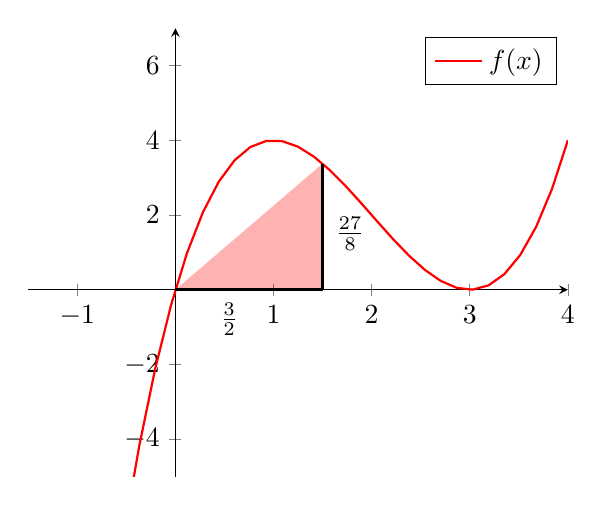
\begin{tikzpicture}   
\begin{axis}[
    axis lines=middle,
    samples=35,
    domain=-1.5:4,
    ymax=7,
    ymin=-5,
    every axis plot/.append style={thick},
]
\addplot[
    color=red,
    name path=A
]
{((\x)*(\x)*(\x))-(6*(\x)*(\x))+(9*(\x))};
\addlegendentry{$f(x)$}

\addplot[draw=none,name path=B] {((27/8)/(3/2))*(\x)};
\addplot[draw=none,name path=C] {0};
\addplot[red,opacity=0.3] fill between[of=B and C,soft clip={domain=0:1.5}];

\addplot[color=black,very thick] coordinates {(1.5,0) (1.5,3.375)};
\addplot[color=black,very thick] coordinates {(0,0) (1.5,0)};

\node[label={0:{$\frac{27}{8}$}},draw=none,inner sep=1pt] at (axis cs:1.5,1.5) {};
\node[label={250:{$\frac{3}{2}$}},draw=none,inner sep=1pt] at (axis cs:0.75,0) {};

\end{axis}
\end{tikzpicture}
\end{center}

\section{Integralrechnung}
\subsection{Stammfunktionen}
\begin{flushleft}
    Stammfunktionen sind Funktionen, die eine Funktion $f$ ergeben, wenn man sie ableitet.
    Also gilt: $F'(x)=f(x)$.

    Allgemein gilt die folgende Regel.
    \begin{align}
        f(x)&=x^n \\
        F(x)&=\frac{x^{n+1}}{n+1}+C, n \in \mathbf{R} - \{-1\}
    \end{align}
    Wenn eine Funktion abgeleitet wird fällt jede Konstante weg, daher gibt es unendlich viele Stammfunktionen, die Konstante wird mit $C$ dargestellt.
\end{flushleft}

\subsection{Bestimmte Integrale}
\begin{flushleft}
    Bei bestimmten Integralen ist immer klar, welches Intervall gesucht ist.
    Also gilt für ein Integral in dem Intervall $[a;b]$ diese Formel:
    \begin{align}
        \int_{a}^{b} f(x) \ dx = [F(x)]_{a}^{b}
    \end{align}
    Außerdem ist die Integralrechnung keine Flächenberechnung, daher werden oft Absolutbeträge genutzt. Damit wird das Ergebnis eines Integrals immer positiv.
    Die Definition des Absolutbetrags sieht so aus:
    \[
        \left | x \right | =
        \begin{cases}
            x, &\text{wenn } x \geq 0 \\
            -x, &\text{sonst}
        \end{cases}
    \]
    Dass die Integralrechnung keine Flächenberechnung ist kann man sich schnell deutlich machen.
    Haben wir beispielsweise die Funktion $f(x)=-x^2+4$ gegeben und wollen diese von $-2$ bis $2$ integrieren, sieht die Fläche, die wir berechnen wollen so aus:
\end{flushleft}

\begin{center}
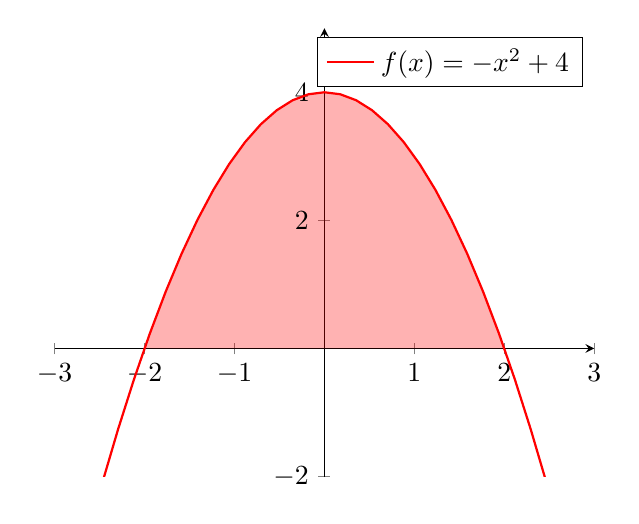
\begin{tikzpicture}
\begin{axis}[
        xmin=-3,
        xmax=3,
        ymax=5,
        ymin=-2,
        domain=-3:3,
        samples=35,
        axis lines=middle,
        %unbound coords=discard,
    ]
    \addplot[red,thick,name path=A] ({\x},{-((\x)*(\x))+4});
    \addlegendentry{\(f(x)=-x^2+4\)}
    
    \addplot[draw=none,name path=B] {0};
    \addplot[red,opacity=0.3] fill between[of=A and B,soft clip={domain=-2:2}];
\end{axis}
\end{tikzpicture}
\end{center}

\begin{flushleft}
    Jetzt bilden wir das Integral und lösen es auf.
    \begin{align}
        &\int_{-2}^{2} -x^2+4 \ dx \\
        = &\left[\frac{-x^3}{3}+4x\right]_{-2}^{2} \\
        = &\left[\frac{-2^3}{3}+4*2-\left(\frac{-(-2)^3}{3}+4(-2)\right)\right] \\
        = &\frac{32}{3}
    \end{align}
    Es gibt keine Probleme. Möchten wir jetzt jedoch von $2$ bis $4$ integrieren, stellen wir etwas komisches fest.
\end{flushleft}

\begin{center}
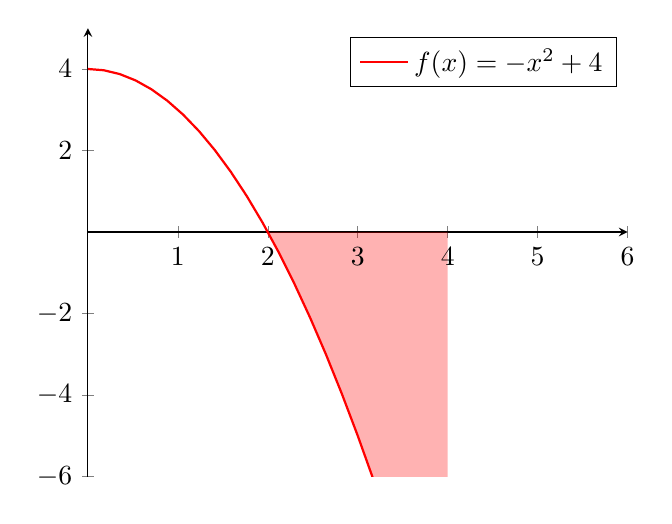
\begin{tikzpicture}
\begin{axis}[
        xmin=0,
        xmax=6,
        ymax=5,
        ymin=-6,
        domain=0:6,
        samples=35,
        axis lines=middle,
        %unbound coords=discard,
    ]
    \addplot[red,thick,name path=A] ({\x},{-((\x)*(\x))+4});
    \addlegendentry{\(f(x)=-x^2+4\)}
    
    \addplot[draw=none,name path=B] {0};
    \addplot[red,opacity=0.3] fill between[of=A and B,soft clip={domain=2:4}];
\end{axis}
\end{tikzpicture}
\end{center}

\begin{flushleft}
    Erstmal das Integral bilden.
    \begin{align}
        &\int_{2}^{4} -x^2+4 \ dx \\
        = &\left[\frac{-x^3}{3}+4x\right]_{2}^{4} \\
        = &\left[\frac{-4^3}{3}+4*4-\left(\frac{-2^3}{3}+4*2\right)\right] \\
        = &\frac{-32}{3}
    \end{align}
    Das Ergebnis ist negativ, obwohl ein negativer Flächeninhalt nicht möglich ist.
    Deshalb nutzen wir, wenn das Ergebnis des Integrals negativ ist -- was vorher geprüft werden sollte -- den Betrag des Ergebnisses.
    \begin{align}
        & \left | \int_{2}^{4} -x^2+4 \ dx \right | \\
        = & \left | \frac{-32}{3} \right | \\
        = &\frac{32}{3}
    \end{align}
\end{flushleft}

\subsection{Flächen zwischen zwei Funktionen}
\begin{flushleft}
    Um die Fläche zwischen den beiden Funktionen $f$ und $g$ ($f \geq g$) im Intervall $[a;b]$ zu berechnen nutzt man diese Formel:
    \begin{align}
        \int_{a}^{b} \left[f(x)-g(x)\right] \ dx
    \end{align}
    Beispiel: $f(x)=-x^2+4$, $g(x)=2$
\end{flushleft}

\begin{center}
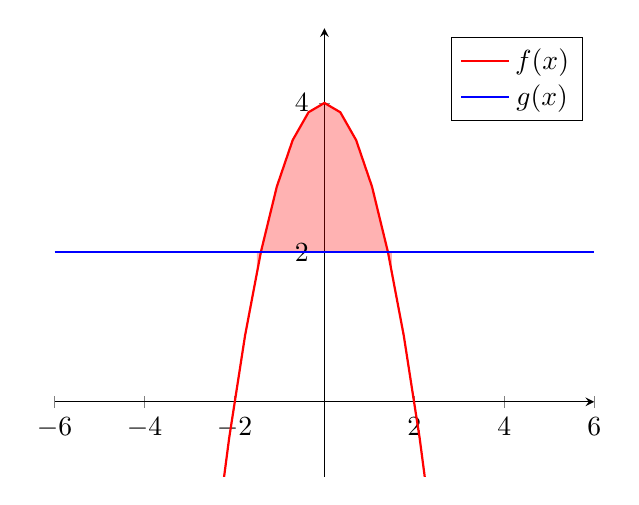
\begin{tikzpicture}
\begin{axis}[
        xmin=-6,
        xmax=6,
        ymax=5,
        ymin=-1,
        domain=-6:6,
        samples=35,
        axis lines=middle,
        %unbound coords=discard,
    ]
    \addplot[red,thick,name path=A] ({\x},{-((\x)*(\x))+4});
    \addlegendentry{\(f(x)\)}
    \addplot[blue,thick,name path=B] ({\x},{2});
    \addlegendentry{\(g(x)\)}
    
    \addplot[red,opacity=0.3] fill between[of=A and B,soft clip={domain=-1.5:1.5}];
\end{axis}
\end{tikzpicture}
\end{center}

\begin{flushleft}
    Um die Fläche zwischen $f$ und $g$ zu bestimmen muss zunächst klar werden, welche Funktion in dem gezeigten Bereich größer ist.
    Hier ist $f > g, [x_1;x_2]$, $x_1$ und $x_2$ stellen hier die Schnittpunkte der beiden Funktionen dar.
    Jetzt darf einfach in die Formel eingesetzt werden, $x_1$ und $x_2$ müssen dafür natürlich erst bestimmt werden, das werden wir in diesem Beispiel jedoch nicht machen.
    \begin{align}
        \int_{x_1}^{x_2} \left[f(x)-g(x)\right] \ dx
    \end{align}
\end{flushleft}

\subsection{Mittelwerte von Funktionen}
\begin{flushleft}
    \textbf{diskrete Mittelwerte}: \newline
    Es wird ein Mittelwert aus einer Menge von Zahlen gebildet. \newline
    \begin{align}
        \{1,3&,5,4\} \\
        \frac{1+3+5+4}{4}&=\frac{13}{4}=3.25
    \end{align}
    \newline
    \textbf{kontinuierliche Mittelwerte}: \newline
    Der Mittelwert wird aus Werten einer Funktion bestimmt. \newline
    \begin{align}
        \bar{m}=\frac{1}{b-a}\int_{a}^{b} f(x) \ dx
    \end{align}
    Beispiel: $f(x)=-x^2+4$
\end{flushleft}

\begin{center}
\begin{tikzpicture}
\begin{axis}[
        xmin=-4,
        xmax=4,
        ymax=5,
        ymin=-1,
        domain=-4:4,
        samples=35,
        axis lines=middle,
        %unbound coords=discard,
    ]
    \addplot[red,thick,name path=A] ({\x},{-((\x)*(\x))+4});
    \addlegendentry{\(f(x)\)}
\end{axis}
\end{tikzpicture}
\end{center}

\begin{flushleft}
    Wir wollen den Mittelwert $\bar{m}$ von $f$ in dem Interval $\left[-2;2\right]$ bestimmen.
    Dafür setzen wir einfach in die Formel ein.
    \begin{align}
        \bar{m}&=\frac{1}{b-a}\int_{a}^{b} f(x) \ dx \\
        \bar{m}&=\frac{1}{2-(-2)}\int_{-2}^{2} -x^2+4 \ dx \\
        \bar{m}&=\frac{1}{4}\int_{-2}^{2} -x^2+4 \ dx \\
        \bar{m}&=\frac{1}{4}\left[\frac{-x^3}{3}+4x\right]_{-2}^{2} \\
        \bar{m}&=\frac{1}{4}\left[\frac{-2^3}{3}+4*2-\left(\frac{-(-2)^3}{3}+4(-2)\right)\right] \\
        \bar{m}&=\frac{1}{4}*\frac{32}{3} \\
        \bar{m}&=\frac{8}{3}
    \end{align}
    Der Mittelwert der Funktion $f$ im Interval $\left[-2;2\right]$ ist also $\frac{8}{3}$.
\end{flushleft}

\begin{center}
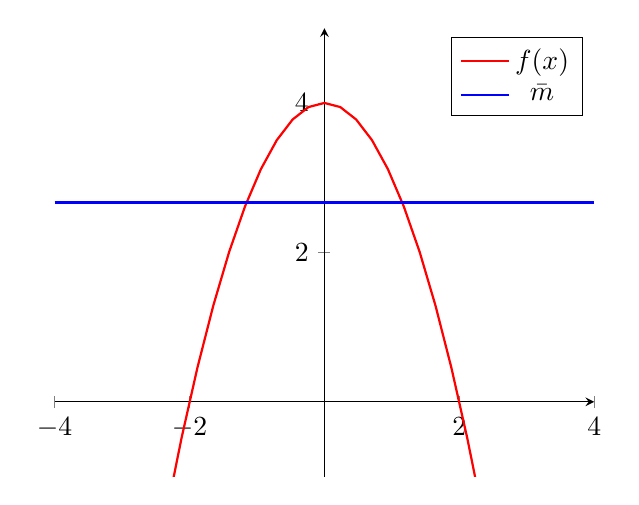
\begin{tikzpicture}
\begin{axis}[
        xmin=-4,
        xmax=4,
        ymax=5,
        ymin=-1,
        domain=-4:4,
        samples=35,
        axis lines=middle,
        %unbound coords=discard,
    ]
    \addplot[red,thick,name path=A] ({\x},{-((\x)*(\x))+4});
    \addlegendentry{\(f(x)\)}
    
    \addplot[blue,thick,name path=B] ({\x},{8/3});
    \addlegendentry{\(\bar{m}\)}
\end{axis}
\end{tikzpicture}
\end{center}

\subsection{Rekonstruktion von Beständen}
\begin{flushleft}
    Bei diesem Aufgabentyp hat man immer eine Funktion (hier: $f$) gegeben, die die momentane Änderungsrate beschreiben soll, also wie stark etwas ansteigt oder fällt.
    Um alle Teilaufgaben vernünftig zu lösen muss man erstmal die Stammfunktion bestimmen:
    \begin{align}
        f(x)&=F'(x) \\
        F(x)&=\int f(x) \ dx
    \end{align}
    Die Konstante $C$, die beim integrieren erscheint sollte in der Aufgabenstellung gegeben sein.
\end{flushleft}

\subsection{Rotationskörper}
\begin{flushleft}
    Rotationskörper, sind Objekte, die sich bilden wenn eine Funktion um eine Achse rotiert.
    Die Rotationsachse wird auch die Figureachse genannt.
    Um allgemein das Volumen eines Rotationskörpers, der durch die Funktion $f$ beschrieben wird zu bestimmen nutzt man diese Formel:
    \begin{align}
        V=\pi\int_{a}^{b}\left[f(x)\right]^2 \ dx
    \end{align}
    Beispiel: $f(x)=x^2$, im Interval $[0;2]$
\end{flushleft}

\begin{center}
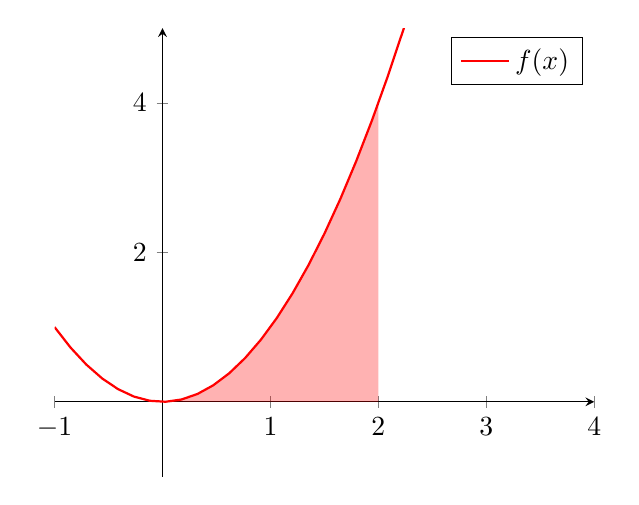
\begin{tikzpicture}
\begin{axis}[
        xmin=-1,
        xmax=4,
        ymax=5,
        ymin=-1,
        domain=-1:4,
        samples=35,
        axis lines=middle,
        %unbound coords=discard,
    ]
    \addplot[red,thick,name path=A] ({\x},{((\x)*(\x))});
    \addlegendentry{\(f(x)\)}
    
    \addplot[draw=none,name path=B] ({\x},{0});
    \addplot[red,opacity=0.3] fill between[of=A and B,soft clip={domain=0:2}];
\end{axis}
\end{tikzpicture}
\end{center}

\begin{flushleft}
    Wenn diese Funktion $f$ um die X-Achse rotiert wird, sieht der Körper, der entsteht in etwa so aus:
\end{flushleft}

% Code von: https://tex.stackexchange.com/questions/191091/function-rotated-about-the-x-axis
\begin{center}
    \def\aDomain{0}
    \def\bDomain{2}

    \def\fcn{\x^2}

    \def\cRange{0}
    \def\dRange{4}

    \def\xGridSteps{8}

    \def\rotationGridSteps{16}

    \def\phi{17}

\begin{tikzpicture}[domain= \aDomain: \bDomain]
    \pgfmathsetmacro\intervalLength{\bDomain - \aDomain}
    \pgfmathsetmacro\xGridStepsize{\intervalLength/\xGridSteps}
    \pgfmathsetmacro\rotationGridStepsize{360/\rotationGridSteps}

    \foreach \theta in {0, \rotationGridStepsize, ..., 180} {
        \tikzset{xyplane/.estyle={cm={
        cos(\phi), 0, sin(\theta)*sin(\phi),
        cos(\theta), (0, 0)}}}
        \draw[xyplane,smooth] plot (\x, \fcn) ;
    }

    \pgfmathsetmacro\nextStep{\aDomain + \xGridStepsize}
    \foreach \x in {\aDomain,\nextStep, ...,\bDomain} {
        \pgfmathsetmacro\xsh{(cos(\phi))*(\x)}
        \pgfmathsetmacro\rad{(\fcn)}        
        \tikzset{xyplane/.estyle={cm={cos(\phi - 90), 0,0,1,(\xsh, 0)}}}        
        \draw[xyplane,black,thin,opacity=1] (0, \rad) arc (90 : 270 : \rad);
    }

    \foreach \theta in {0, \rotationGridStepsize, ..., 180} {
        \tikzset{xyplane/.estyle={cm={cos(\phi), 0, sin(\theta)*sin(\phi),cos(\theta),(0, 0)}}}
        \draw[xyplane,smooth] plot (\x, \fcn) ;
    }

    \foreach \x in {\aDomain, \nextStep, ..., \bDomain}{
        \pgfmathsetmacro\xsh{(cos(\phi))*(\x)}
        \pgfmathsetmacro\rad{(\fcn)}
        \tikzset{xyplane/.estyle={cm={cos(\phi-90),0,0,1, (\xsh, 0)}}}
        \draw[xyplane] (0, -\rad) arc (-90 : 90 : \rad);
    }
\end{tikzpicture}
\end{center}

\begin{flushleft}
    Jetzt interessiert uns das Volumen $V$, das dieser Körper hat.
    Dazu setzen wir unsere Werte in die Formel ein.
    \begin{align}
        V &=\pi\int_{0}^{2}\left[x^2\right]^2 \ dx \\
        V &=\pi\int_{0}^{2} x^4 \ dx \\
        V &=\pi \left[\frac{x^5}{5}\right]_{0}^{2} \\
        V &=\pi \left[\frac{2^5}{5}-\left(\frac{0^5}{5}\right)\right] \\
        V &=\pi \frac{32}{5} \\
        V &=\frac{32\pi}{5}
    \end{align}
    Nun wissen wir, dass das Volumen $V$ unseres Rotationskörpers $\frac{32\pi}{5}$ ist.
\end{flushleft}

\subsection{Uneigentliche Integrale}
\begin{flushleft}
    Uneigentliche Integrale sind bestimmte Integrale mit komplizierteren Integrationsgrenzen.
    Oft wird $-\infty$ oder $+\infty$ in die Integrationsgrenzen eingebaut, es können jedoch auch Integrale mit richtigen Zahlen uneigentlich sein.
\end{flushleft}

\begin{center}
\begin{tikzpicture}
\begin{axis}[
        xmin=0,
        xmax=5,
        ymax=5,
        ymin=0,
        domain=0.05:5,
        samples=35,
        axis y line=left,
        axis x line=bottom,
        restrict y to domain=0:5
        %unbound coords=discard,
    ]
    \addplot[red,thick,name path=A] ({\x},{1/((\x)*(\x))});
    \addlegendentry{\(f(x)=\frac{1}{x^2}\)}
\end{axis}
\end{tikzpicture}
\end{center}

\begin{flushleft}
    Hier sieht man den Plot von $f(x)=\frac{1}{x^2}$.
    Es lässt sich relativ gut erkennen, dass der Wert der Funktion immer größer wird, umso näher man der Y-Achse kommt.
    Entfernt man sich also von der Y-Achse, wird der Wert immer kleiner.
    Mathematisch lässt sich das so ausdrücken:
    \begin{align}
        \lim_{x \to 0} f(x) &= \infty \\
        \lim_{x \to \infty} f(x) &= 0 \\
        \lim_{x \to -\infty} f(x) &= 0
    \end{align}
    Diese Grenzen muss man beachten, wenn man uneigentliche Integrale, wie beispielsweise dieses Integral ausrechnen möchte.
    \begin{align}
        &\int_{1}^{\infty} f(x) \ dx
    \end{align}
    Mit diesem Integral würde man die folgende Fläche berechnen:
\end{flushleft}

\begin{center}
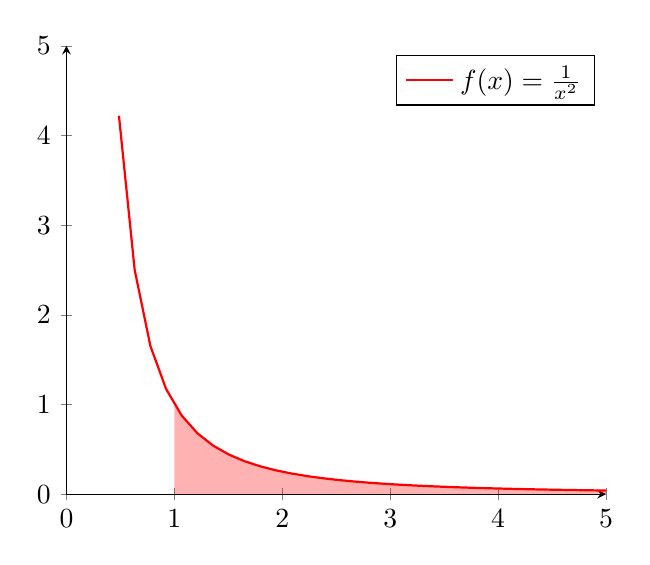
\begin{tikzpicture}
\begin{axis}[
        xmin=0,
        xmax=5,
        ymax=5,
        ymin=0,
        domain=0.05:5,
        samples=35,
        axis y line=left,
        axis x line=bottom,
        restrict y to domain=0:5
        %unbound coords=discard,
    ]
    \addplot[red,thick,name path=A] ({\x},{1/((\x)*(\x))});
    \addlegendentry{\(f(x)=\frac{1}{x^2}\)}
    
    \addplot[draw=none,name path=B] {0};
    \addplot[red,opacity=0.3] fill between[of=A and B,soft clip={domain=1:5}];
\end{axis}
\end{tikzpicture}
\end{center}

\begin{flushleft}
    Wenn man versucht dieses Integral zu berechnen fällt eine Besonderheit auf.
    \begin{align}
        &\int_{1}^{\infty} f(x) \ dx \\
        &\int_{1}^{\infty} \frac{1}{x^2} \ dx \\
        &\int_{1}^{\infty} x^{-2} \ dx \\
        &\left[\frac{x^{-1}}{-1}\right]_{1}^{\infty} \\
        &\left[\frac{-1}{x}\right]_{1}^{\infty}
    \end{align}
    Als obere Grenze kann nicht einfach $\infty$ eingesetzt werden, deshalb suchen wir einen Weg um uns an $\infty$ anzunähern.
    \begin{align}
        &\lim_{b \to \infty} \left[ \frac{-1}{x}\right]_{1}^{b}
    \end{align}
    Jetzt ist es möglich anstatt $\infty$ einfach unsere Variable $b$ einzusetzen und erstmal so weit wie möglich aufzulösen.
    \begin{align}
        &\lim_{b \to \infty} \left[ \frac{-1}{b} - \left(\frac{-1}{1}\right)\right] \\
        &\lim_{b \to \infty} \left( \frac{-1}{b} + 1\right)
    \end{align}
    Nachdem wir so weit wie möglich vereinfacht haben, gucken wir uns jetzt jeden Bestandteil des Ergebnisses an.
    Da unsere Variable $b$ ist, interessieren uns erstmal nur die Terme, in denen $b$ vorkommt.
    $+1$ ist für den Limes irrelevant, da es kein $b$ enthält, $\frac{-1}{b}$ ist jedoch relevant, deshalb müssen wir uns $\frac{-1}{b}$ genauer angucken. \newline
    Dazu müssen wir uns fragen, was passiert, wenn $b$ einen sehr großen Wert annimmt.
    Anhand von ein paar Beispielen kann man das verhalten von $\frac{-1}{b}$ relativ gut verinnerlichen.
    Man kann zur Veranschaulichung einfach ein paar Werte für $b$ einsetzen.
    \begin{align}
        &\frac{-1}{b} \\ 
        \frac{-1}{2} &= -0.5 \\ 
        \frac{-1}{4} &= -0.25 \\ 
        \frac{-1}{8} &= -0.125 \\ 
        \frac{-1}{16} &= -0.0625
    \end{align}
    Wie man relativ gut erkennen kann, geht $\frac{-1}{b}$ immer weiter gegen $0$, desto größer der Wert für $b$ ist.
    Das bedeutet für unsere ursprüngliche Frage, dass dieser Term wegfällt.
    \begin{align}
        \lim_{b \to \infty} &\left( \frac{-1}{b} + 1\right) \\
        &=1 \\
        \int_{1}^{\infty} f(x) \ dx &= 1
    \end{align}
    Nach ein wenig Rechnerei wissen wir also, dass unser uneigentliches Integral, welches eine obere Grenze von $\infty$ hat, nicht den Wert von $\infty$, 
    sondern einen Wert von $1$ hat.
\end{flushleft}

\chapter{Stochastik}

\section{Binomialverteilungen}
\subsection{Definition}
\begin{flushleft}
    Eine Binomialverteilung ist eine diskrete Wahrscheinlichkeitsverteilung. Das bedeutet, dass eine Binomialverteilung
    auf einer kleineren Menge definiert ist. Oft ist diese Menge endlich (${0,1,2,\dots,n}$), sie kann aber auch abzählbar
    unendlich (Bsp.: Menge der natürlichen Zahlen) sein. \\
    Außerdem kennt eine Binomialverteilung nur zwei Versuchsausgänge, Erfolg oder Misserfolg. Solche Experimente werden Bernoulli
    Experimente genannt.
\end{flushleft}

\subsection{Aufgabentypen}
\begin{flushleft}
    Für alle hier beschriebenen Aufgabentypen gilt $n$ als die Anzahl aller Versuchsausgänge, $k$ als die beschränkte Anzahl von
    Versuchsausgängen und $p$ als Erfolgswahrscheinlichkeit. \\
    \textit{Beispiel: Ein Würfel wird 100 mal geworfen, wie hoch ist die Wahrscheinlichkeit, dass 5 Sechsen geworfen werden?} \\
    Hier gilt:
    \begin{align}
        n=100,k=5,p=\frac{1}{6}
    \end{align}
\end{flushleft}

\subsubsection{Bestimmung von P}
\begin{flushleft}
    Der häufigste und einfachste Aufgabentyp ist die Bestimmung von $P$.
    Hierbei verlässt man sich auf eine treue Formel.
    \begin{align}
        P(X=k)=\binom{n}{k} \cdot p^k \cdot (1-p)^{n-k}
    \end{align}
    Kumulierte Wahrscheinlichkeiten berechnet man mit der selben Formel, diese benötigen
    jedoch mehr Aufwand.
    \begin{align}
        P(X \leq 2)=P(X=0)+P(X=1)+P(X=2)
    \end{align}
    Mathematica bietet den $CDF$ Befehl um diese Art der kumulierten Wahrscheinlichkeit auszurechnen.
    Somit lässt sich jeder beliebige Ausdruck in solch einen Ausdruck umformen und mit Mathematica berechnen.
    \begin{align}
        P(X>k) &= 1-P(X \leq k) \\
        P(X \geq k) &= 1-P(X \leq k-1) \\
        P(X<k) &= P(X \leq k-1) \\
        P(k_{1} \leq X \leq k_{2}) &= P(X \leq k_{2})-P(X \leq k_{1}-1)
    \end{align}
\end{flushleft}

\subsubsection{Bestimmung von n}
\begin{flushleft}
    In manchen Aufgaben sind nur $p$ und $k$ gegeben, $n$ muss bestimmt werden.
    Aus der Aufgabenstellung geht dann eine ähnliche Ungleichung hervor (hier: $p=0.6$ und $k=n$):
    \begin{align}
        P(X=n) &\leq 0.01 \\
        \binom{n}{n} \cdot 0.6^n \cdot 0.4^0 &\leq 0.01 \\
        0.6^n &\leq 0.01 \\
        \ln(0.6^n) &\leq \ln(0.01) \\
        n\ln(0.6) &\leq \ln(0.01) \\
        n &\geq \frac{\ln(0.01)}{\ln(0.6)} \approx 9.01 \\
        \geq &\text{, da} \ln(0.6)<0
    \end{align}
    Hier ist also, wie so oft in der Stochastik, die einzige Kunst das Entschlüsseln der Aufgabenstellung.
\end{flushleft}

\subsubsection{Erwartungswert und Standardabweichung}
\begin{flushleft}
    Der Erwartungswert $\mu$ und die Standardabweichung $\sigma$ sind wichtige Bestandteile der Stochastik.
    Glücklicherweise ist es bei Binomialverteilungen relativ einfach $\mu$ und $\sigma$ zu bestimmen.
    \begin{align}
        \mu &= n \cdot p \\
        \sigma &= \sqrt{n \cdot p \cdot (1-p)}
    \end{align}
    Der Erwartungswert ist der Wert, der im Schnitt erwartet wird, wenn ein Experiment oft ausgeführt wird.
    Die Standardabweichung ist die mögliche Abweichung vom Erwartungswert.
    Dieses Interval beschreibt diese Abweichung:
    \begin{align}
        [\mu-\sigma;\mu+\sigma]
    \end{align}
\end{flushleft}

\chapter{Analytische Geometrie}

\section{Vektorrechnung}
\begin{flushleft}
Ein Vektor kann als die Verschiebung eines Punktes gesehen werden.
Dabei kann jedoch ein einzelner Vektor auf eine beliebige Menge von Punkten angewandt werden.
Wenn man den Vektor $\vec{a}$ auf den Punkt $P$ anwendet, bekommt man also einen zweiten Punkt $P'$,
dessen Koordinaten um die Werte des Vektors $\vec{a}$ verschoben wurden.

\begin{align}
    \vec{a} &= \begin{pmatrix} 1 \\ 1 \\ 1 \end{pmatrix} \\
    P &= \left(1,2,3\right) \\
    P' &= \left(1+1,2+1,3+1\right) = \left(2,3,4\right)
\end{align}
\end{flushleft}

\begin{center}
\begin{tikzpicture}
\begin{axis}[
    view={35}{15},
    axis lines=center,
    width=15cm,height=15cm,
    xtick={1,2,3,4,5},ytick={1,2,3,4,5},ztick={1,2,3,4,5},
    xmin=0,xmax=5,ymin=0,ymax=5,zmin=0,zmax=5,
    xlabel={$x$},ylabel={$y$},zlabel={$z$}
]

\addplot3 [only marks] coordinates {(1,2,3) (2,3,4)};
\addplot3 [no marks,densely dashed] coordinates {(1,0,0) (1,2,0) (1,2,3) (1,2,0) (0,2,0)};
\addplot3 [no marks,densely dashed] coordinates {(2,0,0) (2,3,0) (2,3,4) (2,3,0) (0,3,0)};

\node [above left] at (axis cs:1,2,3) {$P(1,2,3)$};
\node [above right] at (axis cs:2,3,4) {$P'(2,3,4)$};
\draw [->,thick] (axis cs:1,2,3) to (axis cs:1.97,2.97,3.97);
\node [above left] at (axis cs:1.5,2.5,3.5) {$\vec{a}$};

\end{axis}
\end{tikzpicture}
\end{center}

\subsection{Ortsvektoren}
\begin{flushleft}   
Ortsvektoren verschieben den Ursprung des Koordinatensystems.
Der Ortsvektor $\overrightarrow{OP}$ hat also die gleichen Koordinaten, wie der Punkt $P$,
da $O=(0,0,0)$ ist.

\begin{align}
    O &= (0,0,0) \\
    P &= (1,2,3) \\
    \overrightarrow{OP} &= \begin{pmatrix} 1 \\ 2 \\ 3 \end{pmatrix}
\end{align}
\end{flushleft}

\begin{center}
\begin{tikzpicture}
\begin{axis}[
    view={35}{15},
    axis lines=center,
    width=15cm,height=15cm,
    xtick={1,2,3,4,5},ytick={1,2,3,4,5},ztick={1,2,3,4,5},
    xmin=-2,xmax=5,ymin=-2,ymax=5,zmin=-2,zmax=5,
    xlabel={$x$},ylabel={$y$},zlabel={$z$}
]

\addplot3 [only marks] coordinates {(0,0,0) (1,2,3)};
\addplot3 [no marks,densely dashed] coordinates {(1,0,0) (1,2,0) (1,2,3)};
\addplot3 [no marks,densely dashed] coordinates {(0,2,0) (1,2,0)};

\node [above right] at (axis cs:1,2,3) {$P(1,2,3)$};
\node [left] at (axis cs:0,0,0) {$O(0,0,0)$};
\draw [->,thick] (axis cs:0,0,0) to (axis cs:0.95,1.95,2.95);
\node [below] at (axis cs:0.3,1.3,2.3) {$\overrightarrow{OP}$};

\end{axis}
\end{tikzpicture}
\end{center}

\subsection{Addition}
\begin{flushleft}
Die Addition von Vektoren ist sehr simpel.
Wenn $\vec{a}$ und $\vec{b}$ addiert werden sollen, werden alle Einträge von $\vec{b}$
zu den Einträgen von $\vec{a}$ addiert.
\begin{align}
    \vec{a} &= \begin{pmatrix} 1 \\ 1 \\ 1 \end{pmatrix} \\
    \vec{b} &= \begin{pmatrix} 2 \\ 3 \\ 4 \end{pmatrix} \\
    \vec{a}+\vec{b} &= \begin{pmatrix} 1+2 \\ 1+3 \\ 1+4 \end{pmatrix} \\
    \vec{a}+\vec{b} &= \begin{pmatrix} 3 \\ 4 \\ 5 \end{pmatrix}
\end{align}
\end{flushleft}

\begin{center}
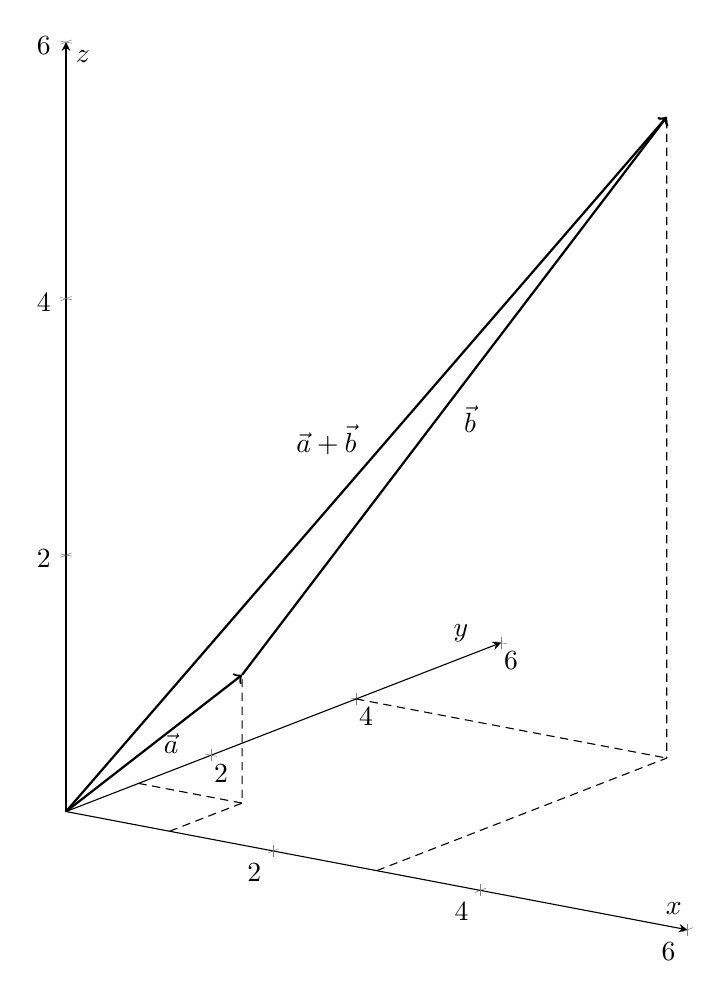
\begin{tikzpicture}
\begin{axis}[
    view={35}{15},
    axis lines=center,
    width=15cm,height=15cm,
    xtick={2,4,6},ytick={2,4,6},ztick={2,4,6},
    xmin=0,xmax=6,ymin=0,ymax=6,zmin=0,zmax=6,
    xlabel={$x$},ylabel={$y$},zlabel={$z$}
]

\addplot3 [no marks,densely dashed] coordinates {(1,0,0) (1,1,0) (1,1,1)};
\addplot3 [no marks,densely dashed] coordinates {(0,1,0) (1,1,0)};

\addplot3 [no marks,densely dashed] coordinates {(3,0,0) (3,4,0) (3,4,5)};
\addplot3 [no marks,densely dashed] coordinates {(0,4,0) (3,4,0)};

\draw [->,thick] (axis cs:0,0,0) to (axis cs:1,1,1);
\node [right] at (axis cs:0.5,0.5,0.5) {$\vec{a}$};

\draw [->,thick] (axis cs:1,1,1) to (axis cs:3,4,5);
\node [below right] at (axis cs:2,2.5,3) {$\vec{b}$};

\draw [->,thick] (axis cs:0,0,0) to (axis cs:3,4,5);
\node [above left] at (axis cs:1.5,2,2.5) {$\vec{a}+\vec{b}$};

\end{axis}
\end{tikzpicture}
\end{center}

\subsection{Multiplikation}
\begin{flushleft}    
Ein Vektor kann mit einer Zahl $r \in \mathbb{R}$ multipliziert werden.
Ähnlich wie bei der Addition werden hier alle Einträge eines Vektors mit $r$ multipliziert.

\begin{align}
    \vec{a} &= \begin{pmatrix} 1 \\ 2 \\ 3 \end{pmatrix} \\
    r &= 2 \\
    2\vec{a} &= \begin{pmatrix} 2 \cdot 1 \\ 2 \cdot 2 \\ 2 \cdot 3 \end{pmatrix} = \begin{pmatrix} 2 \\ 4 \\ 6 \end{pmatrix}
\end{align}
\end{flushleft}

\begin{center}
\begin{tikzpicture}
\begin{axis}[
    view={35}{15},
    axis lines=center,
    width=15cm,height=15cm,
    xtick={2,4,6},ytick={2,4,6},ztick={2,4,6},
    xmin=0,xmax=6,ymin=0,ymax=6,zmin=0,zmax=6,
    xlabel={$x$},ylabel={$y$},zlabel={$z$}
]

\addplot3 [no marks,densely dashed] coordinates {(1,0,0) (1,2,0) (1,2,3)};
\addplot3 [no marks,densely dashed] coordinates {(0,2,0) (1,2,0)};

\addplot3 [no marks,densely dashed] coordinates {(2,0,0) (2,4,0) (2,4,6)};
\addplot3 [no marks,densely dashed] coordinates {(0,4,0) (2,4,0)};

\draw [->,thick,red] (axis cs:1,2,3) to (axis cs:2,4,6);
\node [below right] at (axis cs:1.5,3,4.5) {$2\vec{a}$};

\draw [->,thick,blue] (axis cs:0,0,0) to (axis cs:1,2,3);
\node [right] at (axis cs:0.5,1,1.5) {$\vec{a}$};

\end{axis}
\end{tikzpicture}
\end{center}

\begin{flushleft}
Der Vektor $\vec{a}$ wird hier um $r$ verlängert.
In diesem Beispiel wird $\vec{a}$ also doppelt so lang, da $r=2$ ist.
Falls $\left| r \right| < 1$ ist, wird der Vektor $\vec{a}$ also verkürzt.

\begin{align}
    \vec{a} &= \begin{pmatrix} 1 \\ 2 \\ 3 \end{pmatrix} \\
    r &= \frac{1}{2} \\
    \frac{1}{2} \vec{a} &= \begin{pmatrix} \frac{1}{2} \cdot 1 \\ \frac{1}{2} \cdot 2 \\ \frac{1}{2} \cdot 3 \end{pmatrix} = \begin{pmatrix} \frac{1}{2} \\ 1 \\ \frac{3}{2} \end{pmatrix}
\end{align}
\end{flushleft}

\begin{center}
\begin{tikzpicture}
\begin{axis}[
    view={35}{15},
    axis lines=center,
    width=15cm,height=15cm,
    xtick={2,4,6},ytick={2,4,6},ztick={2,4,6},
    xmin=0,xmax=6,ymin=0,ymax=6,zmin=0,zmax=6,
    xlabel={$x$},ylabel={$y$},zlabel={$z$}
]

\addplot3 [no marks,densely dashed] coordinates {(1,0,0) (1,2,0) (1,2,3)};
\addplot3 [no marks,densely dashed] coordinates {(0,2,0) (1,2,0)};

\addplot3 [no marks,densely dashed] coordinates {(0.5,0,0) (0.5,1,0) (0.5,1,1.5)};
\addplot3 [no marks,densely dashed] coordinates {(0,1,0) (0.5,1,0)};

\draw [->,thick,blue] (axis cs:0,0,0) to (axis cs:0.5,1,1.5);
\node [right] at (axis cs:0.25,0.5,0.75) {$\frac{1}{2}\vec{a}$};

\draw [->,thick,red] (axis cs:0.5,1,1.5) to (axis cs:1,2,3);
\node [below right] at (axis cs:0.75,1.5,2.25) {$\vec{a}$};

\end{axis}
\end{tikzpicture}
\end{center}

\begin{flushleft}
Nach dem selben Prinzip wird die Richtung von $\vec{a}$ getauscht, wenn $r < 0$ ist.
\end{flushleft}

\begin{center}
\begin{tikzpicture}
\begin{axis}[
    view={35}{15},
    axis lines=center,
    width=15cm,height=15cm,
    xtick={1,2,3,4},ytick={1,2,3,4},ztick={1,2,3,4},
    xmin=0,xmax=4,ymin=0,ymax=4,zmin=0,zmax=4,
    xlabel={$x$},ylabel={$y$},zlabel={$z$}
]

\addplot3 [no marks,densely dashed] coordinates {(1,0,0) (1,2,0) (1,2,3)};
\addplot3 [no marks,densely dashed] coordinates {(0,2,0) (1,2,0)};

\addplot3 [no marks,densely dashed] coordinates {(0.5,0,0) (0.5,1,0) (0.5,1,1.5)};
\addplot3 [no marks,densely dashed] coordinates {(0,1,0) (0.5,1,0)};

\draw [->,thick,red] (axis cs:0,0,0) to (axis cs:1,2,3);
\node [below right,red] at (axis cs:0.25,0.5,0.75) {$\vec{a}$};

\draw [->,thick,blue] (axis cs:1,2,3) to (axis cs:0.5,1,1.5);
\node [right,blue] at (axis cs:0.75,1.5,2.25) {$\frac{-1}{2}\vec{a}$};

\end{axis}
\end{tikzpicture}
\end{center}

\begin{flushleft}
Wenn $\vec{a}$ mit $-1$ multipliziert wird, entsteht sein Gegenvektor $-\vec{a}$,
der die gleiche länge wie $\vec{a}$ hat aber in die andere Richtung zeigt.
\end{flushleft}

\begin{center}
\begin{tikzpicture}
\begin{axis}[
    view={35}{15},
    axis lines=center,
    width=15cm,height=15cm,
    xtick={1,2,3,4},ytick={1,2,3,4},ztick={1,2,3,4},
    xmin=0,xmax=4,ymin=0,ymax=4,zmin=0,zmax=4,
    xlabel={$x$},ylabel={$y$},zlabel={$z$}
]

\addplot3 [no marks,densely dashed] coordinates {(1,0,0) (1,2,0) (1,2,3)};
\addplot3 [no marks,densely dashed] coordinates {(0,2,0) (1,2,0)};

\draw [->,thick,red] (axis cs:0,0,0) to (axis cs:1,2,3);
\node [below right,red] at (axis cs:0.5,1,1.5) {$\vec{a}$};

\draw [->,thick,blue] (axis cs:1,2,3) to (axis cs:0,0,0);
\node [above left,blue] at (axis cs:0.5,1,1.5) {$-\vec{a}$};

\end{axis}
\end{tikzpicture}
\end{center}

\subsection{Subtraktion}
\begin{flushleft}
Die Subtraktion zweier Vektoren ist die Addition des einen Vektor mit dem Gegenvektor des anderen.
Es gilt also:

\begin{align}
    \vec{a} &= \begin{pmatrix} 1 \\ 1 \\ 1 \end{pmatrix} \\
    \vec{b} &= \begin{pmatrix} 2 \\ 3 \\ 4 \end{pmatrix} \\
    \vec{a}-\vec{b} &= \vec{a}+\left(-\vec{b}\right) \\
    \vec{a}-\vec{b} &= \begin{pmatrix} 1 \\ 1 \\ 1 \end{pmatrix}+\left[\begin{pmatrix}-2 \\ -3 \\ -4\end{pmatrix}\right] \\
    \vec{a}-\vec{b} &= \begin{pmatrix} -1 \\ -2 \\ -3 \end{pmatrix}
\end{align}
\end{flushleft}

\subsection{Skalarprodukt}
\begin{flushleft}
Allgemein geht es beim Skalarprodukt um die Multiplikation zweier Vektoren.

Es gilt:
\begin{align}
    \vec{a}\cdot\vec{b}=\begin{pmatrix} a_1 \\ a_2 \\ a_3 \end{pmatrix}\cdot\begin{pmatrix} b_1 \\ b_2 \\ b_3 \end{pmatrix}=a_1 b_1+a_2 b_2+a_3 b_3
\end{align}

Das Skalarprodukt zweier Vektoren ist auch nützlich um herauszufinden ob diese Vektoren zueinander
orthogonal sind.

Ein Vektor $\vec{a}$ ist nämlich orthogonal zu einem anderen Vektor $\vec{b}$, wenn:
\begin{align}
    \vec{a}\cdot\vec{b}=0
\end{align}
ist.
\end{flushleft}

\subsubsection{Herleitung}
\begin{flushleft}
Damit $\vec{a}\perp\vec{b}$ gilt, kann man $\vec{a}$ und $\vec{b}$ als Katheten eines rechtwinkligen Dreiecks sehen.
Somit ergibt sich für die Hypotenuse $\vec{b}-\vec{a}$.
Wenn jetzt der Satz des Pythagoras gilt, gilt auch $\vec{a}\perp\vec{b}$.
Konkret bedeutet das so viel:
\begin{align}
    \vec{a}&\perp\vec{b} \\
    |\vec{a}|^2+|\vec{b}|^2&=|\vec{b}-\vec{a}|^2
\end{align}

Für den ersten Teil der Gleichung ergibt sich so:
\begin{align}
    a_1^2+a_2^2+a_3^2+b_1^2+b_2^2+b_3^2
\end{align}

Der zweite Teil sieht so aus:
\begin{align}
    &\left(b_1-a_1\right)^2+\left(b_2-a_2\right)^2+\left(b_3-a_3\right)^2 \\
    \Leftrightarrow &b_1^2-2b_1a_1+a_1^2+b_2^2-2b_2a_2+a_2^2+b_3^2-2b_3a_3+a_3^2
\end{align}

Hier sieht man relativ klar, dass der erste Term nur gleich dem zweiten sein kann, wenn:
\begin{align}
    -2b_1a_1-2b_2a_2-2b_3a_3=0
\end{align}
ist, da der erste Term im zweiten enthalten ist:
\begin{align}
    \mathbf{b_1^2}-2b_1a_1+\mathbf{a_1^2}+\mathbf{b_2^2}-2b_2a_2+\mathbf{a_2^2}+\mathbf{b_3^2}-2b_3a_3+\mathbf{a_3^2}
\end{align}

Umgeformt sieht das ganze so aus:
\begin{align}
    a_1b_1+a_2b_2+a_3b_3=0
\end{align}

Deswegen gilt also:
\begin{align}
    \vec{a}\cdot\vec{b}=\begin{pmatrix} a_1 \\ a_2 \\ a_3 \end{pmatrix}\cdot\begin{pmatrix} b_1 \\ b_2 \\ b_3 \end{pmatrix}=a_1 b_1+a_2 b_2+a_3 b_3
\end{align}
\end{flushleft}

\subsubsection{Winkel zwischen Vektoren}
\begin{flushleft}
Um den Winkel $\theta$ zwischen $\vec{a}$ und $\vec{b}$ zu berechnen benötigt man die folgende Formel:
\begin{align}
    \cos\theta = \frac{\vec{a}\cdot\vec{b}}{|\vec{a}||\vec{b}|}
\end{align}

% TODO: Herleitung, welcher Winkel wird berechnet?
\end{flushleft}

\subsection{Geraden im Raum}
\begin{flushleft}
Eine Gerade $g$ im Raum besteht aus einem Stützvektor $\vec{v}$ und einem Richtungsvektor $\vec{r}$.

\begin{align}
    g\colon\vec{x}=\vec{v}+t\cdot\vec{r}
\end{align}
\end{flushleft}

% TODO: Geradengleichungen aufstellen

\subsubsection{Punkte einer Geraden bestimmen}
\begin{flushleft}
Beispielhaft ist hier die Gerade $g$ wie folgt definiert:
\begin{align}
    g\colon\vec{x}=\begin{pmatrix} 1 \\ 1 \\ 1 \end{pmatrix}+t\cdot\begin{pmatrix} 1 \\ 1 \\ 1 \end{pmatrix}
\end{align}

Um verschiedene Punkte zu bestimmen, die auf der Geraden liegen muss man bloß einen Wert für $t$ einsetzen:
\begin{align}
    \vec{x}_0=\begin{pmatrix} 1 \\ 1 \\ 1 \end{pmatrix}+0\cdot\begin{pmatrix} 1 \\ 1 \\ 1 \end{pmatrix}=\begin{pmatrix} 1 \\ 1 \\ 1 \end{pmatrix} \\
    \vec{x}_1=\begin{pmatrix} 1 \\ 1 \\ 1 \end{pmatrix}+1\cdot\begin{pmatrix} 1 \\ 1 \\ 1 \end{pmatrix}=\begin{pmatrix} 2 \\ 2 \\ 2 \end{pmatrix}
\end{align}
\end{flushleft}

\subsubsection{Punktproben}
\begin{flushleft}
Wenn man prüfen möchte ob der Punkt $P(1|1|1)$ auf der Geraden:
\begin{align}
    g\colon\vec{x}=\begin{pmatrix} 1 \\ 1 \\ 1 \end{pmatrix}+t\cdot\begin{pmatrix} 1 \\ 1 \\ 1 \end{pmatrix}
\end{align}
liegt, setzt man den Ortsvektor des Punktes $P$ in die Gerade $g$ ein:
\begin{align}
    \begin{pmatrix} 1 \\ 1 \\ 1 \end{pmatrix}=\begin{pmatrix} 1 \\ 1 \\ 1 \end{pmatrix}+t\cdot\begin{pmatrix} 1 \\ 1 \\ 1 \end{pmatrix}
\end{align}

Hier wird schnell klar, dass der Punkt $P(1|1|1)$ für $t=0$ auf der Geraden $g$ liegt, da der Richtungsvektor für $t=0$ wegfällt und der Stützvektor und der Ortsvektor zum Punkt $P$ identisch sind.

Der allgemeine Lösungsansatz ist jedoch ein Gleichungsystem zu bilden:
\begin{align}
    1&=1+t \label{eins} \\
    1&=1+t \label{zwei} \\
    1&=1+t \label{drei}
\end{align}
Das LGS besteht aus den drei Gleichungen \eqref{eins}, \eqref{zwei} und \eqref{drei}.
Da alle Gleichungen identisch sind, reicht es hier eine beliebige Gleichung nach $t$ aufzulösen:
\begin{align}
    1&=1+t \\
    \Leftrightarrow 0&=t
\end{align}
Dieser Lösungsweg zeigt auch, dass der Punkt $P(1|1|1)$ für $t=0$ auf der Geraden $g$ liegt.
\end{flushleft}

\subsubsection{Orthogonalität}
\begin{flushleft}
Möchte man eine Gerade $h$ finden, die zu einer anderen Geraden $g$ orthogonal verläuft, müssen die Richtungsvektoren beider Geraden orthogonal zueinander sein.

Um eine Gerade zu finden, die orthogonal zu der Geraden:
\begin{align}
    g\colon\vec{x}=\begin{pmatrix} 1 \\ 1 \\ 1 \end{pmatrix}+t\cdot\begin{pmatrix} 1 \\ 1 \\ 1 \end{pmatrix}
\end{align}
verläuft, muss man einen Vektor $\vec{r_h}$ finden, der orthogonal zu dem Richtungsvektor $\vec{r_g}$ von $g$ ist:
\begin{align}
    \vec{r_h}&\perp\vec{r_g} \\
    \Leftrightarrow \vec{r_h}\cdot\vec{r_g}&=0 \\
    \Leftrightarrow \begin{pmatrix} r_1 \\ r_2 \\ r_3 \end{pmatrix}\cdot\begin{pmatrix} 1 \\ 1 \\ 1 \end{pmatrix}&=0 \\
    \Leftrightarrow r_1+r_2+r_3&=0 \\
    \Leftrightarrow r_1&=-r_2-r_3 \\
    \Leftrightarrow r_2&=-r_1-r_3 \\
    \Leftrightarrow r_3&=-r_1-r_2
\end{align}
Nun hat man eine Gleichung mit drei Unbekannten, deshalb kann man zwei dieser Unbekannten frei wählen, wählt man also $r_1=1$ und $r_2=2$ ergibt sich die folgende Gleichung für $h$:
\begin{align}
    r_1&=1 \\
    r_2&=2 \\
    r_3&=-1-2=-3 \\
    \vec{r_h}&=\begin{pmatrix} 1 \\ 2 \\ -3 \end{pmatrix} \\
    h\colon\vec{x}&=\begin{pmatrix} 1 \\ 1 \\ 1 \end{pmatrix}+s\cdot\begin{pmatrix} 1 \\ 2 \\ -3 \end{pmatrix}
\end{align}
\end{flushleft}

\subsection{Ebenen im Raum}
\begin{flushleft}
Eine Ebene im Raum kann durch verschiedene Formen dargestellt werden.
Man unterscheidet zwischen Parameter-, Normalen-, und Koordinatenform.
\end{flushleft}

\subsubsection{Parameterform}
\begin{flushleft}
Eine Ebene $E$ in der Parameterform hat einen Stützvektor $\vec{s}$ und zwei Spannvektoren $\vec{u}$ und $\vec{v}$, die keine Vielfachen von einander sind:
\begin{align}
    E\colon\vec{x}=\vec{s}+t\vec{u}+s\vec{v} \quad t,s\in\mathbb{R}
\end{align}
\end{flushleft}

% TODO: Ebenengleichungen aufstellen

\subsubsection{Normalenform}
\begin{flushleft}
Eine Ebene $E$ in der Normalenform besteht aus einem Normalenvektor $\vec{n}$, der senkrecht zur Ebene steht, und einem Stützvektor $\vec{p}$:
\begin{align}
    E\colon\vec{n}\cdot\left(\vec{x}-\vec{p}\right)=0
\end{align}
\end{flushleft}

% TODO: Normalen-, Koordinatengleichungen aufstellen

\subsubsection{Koordinatenform}
\begin{flushleft}
Die Koordinatenform ist eine Erweiterung der Normalenform:
\begin{align}
    \vec{n}\cdot\left(\vec{x}-\vec{p}\right)&=0 \\
    \Leftrightarrow \vec{n}\cdot\vec{x}-\vec{n}\cdot\vec{p}&=0 \\
    \Leftrightarrow \vec{n}\cdot\vec{x}&=\vec{n}\cdot\vec{p} \\
    \Leftrightarrow \begin{pmatrix}n_1 \\ n_2 \\ n_3 \end{pmatrix}\cdot\begin{pmatrix}x_1 \\ x_2 \\ x_3 \end{pmatrix}&=\vec{n}\cdot\vec{p} \\
    \Leftrightarrow n_1x_1+n_2x_2+n_3x_3&=d \quad n_1,n_2,n_3,d\in\mathbb{R}
\end{align}

Eine Ebene $E$ in der Koordinatenform besteht also aus den Koordinaten $n_1, n_2, n_3$ des Normalenvektors $\vec{n}$ und dem Wert $d$, der sich aus $\vec{n}\cdot\vec{p}$ ergibt:
\begin{align}
    E\colon n_1x_1+n_2x_2+n_3x_3&=d \quad n_1,n_2,n_3,d\in\mathbb{R}
\end{align}
\end{flushleft}

\subsection{Schnittpunkte zwischen Geraden}
\begin{flushleft}
Die Schnittpunkte zwischen einer Geraden $g$ und einer anderen Geraden $h$ kann man herausfinden indem man beide Geraden gleichsetzt.
\begin{align}
    g\colon\vec{x}&=\begin{pmatrix} 1 \\ 1 \\ 1 \end{pmatrix}+t\begin{pmatrix} 1 \\ 1 \\ 1 \end{pmatrix} \\
    h\colon\vec{x}&=\begin{pmatrix} 1 \\ 1 \\ 1 \end{pmatrix}+s\begin{pmatrix} 1 \\ 2 \\ 1 \end{pmatrix} \\
    g&=h \\
    \begin{pmatrix} 1 \\ 1 \\ 1 \end{pmatrix}+t\begin{pmatrix} 1 \\ 1 \\ 1 \end{pmatrix}&=\begin{pmatrix} 1 \\ 1 \\ 1 \end{pmatrix}+s\begin{pmatrix} 1 \\ 2 \\ 1 \end{pmatrix}
\end{align}

Aus den Koordinaten $x_1,x_2,x_3$ ergibt sich ein lineares Gleichungssystem aus drei Gleichungen:
\begin{align}
    \text{I}\colon& 1+t=1+s \\
    \text{II}\colon& 1+t=1+2s \\
    \text{III}\colon& 1+t=1+s
\end{align}

Nun muss das LGS gelöst werden ($III$ wurde entfernt, da $I$=$III$):
\begin{align}
    \text{I}\colon& 1+t=1+s \\
    \text{II}\colon& 1+t=1+2s \\
    \text{Schritt 1}& \\
    \text{I}'\colon& t=s \\
    \text{II}\colon& 1+t=1+2s \\
    \text{Schritt 2}& \\
    \text{I}'\colon& t=s \\
    \text{II}'\colon& 1+s=1+2s \\
    \text{Schritt 3}& \\
    \text{I}'\colon& t=s \\
    \text{II}''\colon& 1=1+s \\
    \text{Schritt 4}& \\
    \text{I}'\colon& t=s \\
    \text{II}'''\colon& 0=s \\
    \text{Lösung}& \\
    &t=s=0
\end{align}

Hier ist der einzige Schnittpunkt der Stützvektor zum Punkt $S(1|1|1)$ beider Geraden.

Zwei Geraden können:
\begin{enumerate}
    \item {windschief verlaufen,}
    \item {parallel verlaufen,}
    \item {einen Schnittpunkt haben.}
\end{enumerate}
\end{flushleft}

\subsection{Schnittpunkte zwischen Gerade und Ebene}
\subsubsection{Ebene in Parameterform}
\begin{flushleft}
Liegt eine Ebene in Parameterform vor, können Gerade und Ebene gleichgesetzt werden.
Beispielsweise kann man die Gerade $g$ gleich der Ebene $E$ setzen:
\begin{align}
    g\colon\vec{x}&=\begin{pmatrix} 1 \\ 1 \\ 1 \end{pmatrix}+t\begin{pmatrix} 1 \\ 1 \\ 1 \end{pmatrix} \\
    E\colon\vec{x}&=\begin{pmatrix} 1 \\ 1 \\ 1 \end{pmatrix}+r\begin{pmatrix} 2 \\ 1 \\ 1 \end{pmatrix}+s\begin{pmatrix} 1 \\ 2 \\ 1 \end{pmatrix} \\
    \begin{pmatrix} 1 \\ 1 \\ 1 \end{pmatrix}+t\begin{pmatrix} 1 \\ 1 \\ 1 \end{pmatrix}&=\begin{pmatrix} 1 \\ 1 \\ 1 \end{pmatrix}+r\begin{pmatrix} 2 \\ 1 \\ 1 \end{pmatrix}+s\begin{pmatrix} 1 \\ 2 \\ 1 \end{pmatrix} \\
    \text{I}\colon& 1+t=1+2r+s \\
    \text{II}\colon& 1+t=1+r+2s \\
    \text{III}\colon& 1+t=1+r+s \\
    \text{Schritt 1}& \\
    \text{I}\colon& 1+t=1+2r+s \\
    \text{II}'\colon& 0=s \\
    \text{III}\colon& 1+t=1+r+s \\
    \text{Schritt 2}& \\
    \text{I}'\colon& 0=r \\
    \text{II}'\colon& 0=s \\
    \text{III}\colon& 1+t=1+r+s \\
    \text{Schritt 3}& \\
    \text{I}'\colon& 0=r \\
    \text{II}'\colon& 0=s \\
    \text{III}'\colon& 1+t=1 \Leftrightarrow t=0
\end{align}

Die Gerade $g$ schneidet die Ebene $E$ für $t=r=s=0$ im Punkt $S(1|1|1)$.
\end{flushleft}

\subsection{Schnittpunkte zwischen Ebenen}
% TODO: Schnittpunkte zwischen Ebenen

\section{Matrizen}
\begin{flushleft}
Matrizen sind sehr nützlich um viele verschiedene Werte in einen Kontext zu bringen.
So lassen sich beispielsweise ein- oder mehrstufige Prozesse durch Matrizen darstellen.
\end{flushleft}

\subsection{Einstufige Prozesse}
\begin{flushleft}   
Beispielsweise können durch die Mischung von Kaffepulver, Wasser und Milch unterschiedliche Kaffesorten produziert werden:
\end{flushleft}

\begin{center}
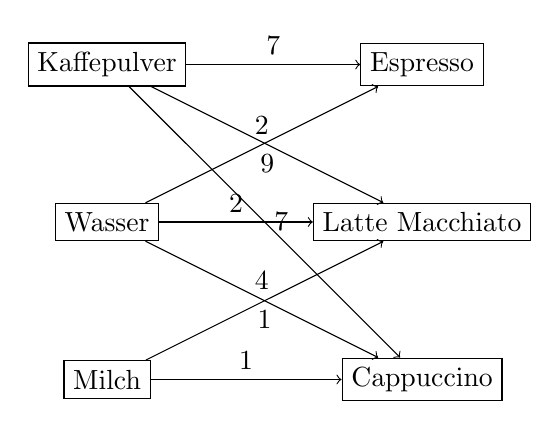
\begin{tikzpicture}
    \node[shape=rectangle,draw=black] (K) at (0,0) {Kaffepulver};
    \node[shape=rectangle,draw=black] (W) at (0,-2) {Wasser};
    \node[shape=rectangle,draw=black] (M) at (0,-4) {Milch};
    \node[shape=rectangle,draw=black] (E) at (4,0) {Espresso};
    \node[shape=rectangle,draw=black] (L) at (4,-2) {Latte Macchiato};
    \node[shape=rectangle,draw=black] (C) at (4,-4) {Cappuccino};

    \path [->] (K) edge node[above] {$7$} (E);
    \path [->] (K) edge node[below] {$9$} (L);
    \path [->] (K) edge node[above,right] {$7$} (C);
    \path [->] (W) edge node[above] {$2$} (E);
    \path [->] (W) edge node[above] {$2$} (L);
    \path [->] (W) edge node[above] {$4$} (C);
    \path [->] (M) edge node[below] {$1$} (L);
    \path [->] (M) edge node[above] {$1$} (C);
\end{tikzpicture}
\end{center}

\begin{center}
\begin{tabular}{c|c|c|c}
& Espresso & Latte Macchiato & Cappuccino \\
\hline
Kaffepulver & 7 & 9 & 7 \\
\hline
Wasser & 2 & 2 & 4 \\
\hline
Milch & 0 & 1 & 1 \\
\end{tabular}
\end{center}

\begin{flushleft}
Dieser Prozess kann durch eine Matrix $A$ dargestellt werden:
\begin{align}
    A = \begin{pmatrix}
        7 & 9 & 7 \\
        2 & 2 & 4 \\
        0 & 1 & 1
    \end{pmatrix}
\end{align}

Um den Bedarf an Kaffepulver, Wasser und Milch für 20 Tassen Espresso, 30 Tassen Latte Macchiato und 15 Tassen Cappuccino zu errechnen,
kann man nun die Matrix $A$ mit dem Vektor $\vec{r}$ multiplizieren, der die gewünschten Werte enthält,
so bekommt man einen anderen Vektor $\vec{s}$, der den Bedarf enthält:
\begin{align}
    A\cdot\vec{r}&=\vec{s} \\
    \begin{pmatrix}
        7 & 9 & 7 \\
        2 & 2 & 4 \\
        0 & 1 & 1
    \end{pmatrix}\cdot
    \begin{pmatrix}
        20 \\
        30 \\
        15
    \end{pmatrix}&=\vec{s}
\end{align}

Aber wie multipliziert man eine Matrix mit einem Vektor?
\newline

Bei einer Matrixmultiplikation sind die Formen der beiden zu multiplizierenden Matrizen zu beachten.
Grundlegend gilt, dass jeder Vektor eine Matrix ist.

Die Matrix $A$ ist hier eine Matrix der Form 3x3, also eine quadratische Matrix, da sie drei Spalten und drei Zeilen hat.
Der Vektor $\vec{r}$ ist hier eine 3x1-Matrix.

Eine Matrix ist immer dann quadratisch, wenn die Anzahl von Spalten gleich der Anzahl von Zeilen ist.

Allgemein dürfen zwei Matrizen $A$ und $B$ nur miteinander multipliziert werden, wenn die Anzahl der Spalten, der Matrix $A$, der Anzahl der Reihen der Matrix $B$ entspricht.

Schaut man sich also die Formen von $A$ und $\vec{r}$ an, sieht man, dass die inneren Werte der beiden Formen gleich sein müssen: 3x\underline{\textbf{3} \textbf{3}}x1.
\newline

Eine Matrixmultiplikation kann man vereinfacht so betrachten, dass die zweite Matrix auf die erste geklappt wird.
Dann wird für jede Zeile das Skalarprodukt gebildet:
\end{flushleft}

\begin{center}
\begin{tabular}{r|l}
& \color{red} 20 \\
& \color{green} 30 \\
& \color{blue} 15 \\
\hline
\color{red} 7 \space \color{green} 9 \space \color{blue} 7 & $7*20+9*30+7*15=515$ \\
\color{red} 2 \space \color{green} 2 \space \color{blue} 4 & $2*20+2*30+4*15=160$ \\
\color{red} 0 \space \color{green} 1 \space \color{blue} 1 & $0*20+1*30+1*15=45$
\end{tabular}
\end{center}

\begin{flushleft}
Das Ergebnis der Multiplikation ist also der Vektor $\vec{s}$:
\begin{align}
    \vec{s}=\begin{pmatrix}
        515 \\
        160 \\
        45
    \end{pmatrix}
\end{align}
\end{flushleft}

\subsection{Zweistufige Prozesse}
\label{subsec:2proc}
\begin{flushleft}
Beispielsweise können verschiedene Eissorten aus Milch $M$, Zucker $Z$ und Früchten $F$ produziert werden.
Bei der Herstellung werden jedoch erst die Zwischenprodukte $S_1$ und $S_2$ produziert, bevor die Endprodukte $E_1$ und $E_2$ produziert werden können.
\end{flushleft}

\begin{center}
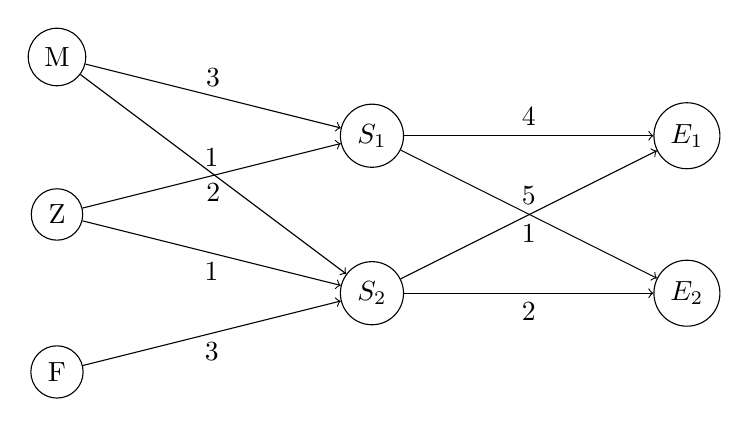
\begin{tikzpicture}
    \node[shape=circle,draw=black] (M) at (0,0) {M};
    \node[shape=circle,draw=black] (Z) at (0,-2) {Z};
    \node[shape=circle,draw=black] (F) at (0,-4) {F};
    \node[shape=circle,draw=black] (S1) at (4,-1) {$S_1$};
    \node[shape=circle,draw=black] (S2) at (4,-3) {$S_2$};
    \node[shape=circle,draw=black] (E1) at (8,-1) {$E_1$};
    \node[shape=circle,draw=black] (E2) at (8,-3) {$E_2$};

    \path [->] (M) edge node[above] {$3$} (S1);
    \path [->] (M) edge node[below] {$2$} (S2);
    \path [->] (Z) edge node[above] {$1$} (S1);
    \path [->] (Z) edge node[below] {$1$} (S2);
    \path [->] (F) edge node[below] {$3$} (S2);
    \path [->] (S1) edge node[above] {$4$} (E1);
    \path [->] (S1) edge node[above] {$5$} (E2);
    \path [->] (S2) edge node[below] {$1$} (E1);
    \path [->] (S2) edge node[below] {$2$} (E2);
\end{tikzpicture}
\end{center}

\begin{center}
\begin{tabular}{c|c|c}
& $S_1$ & $S_2$ \\
\hline
M & 3 & 2 \\
\hline
Z & 1 & 1 \\
\hline
F & 0 & 3
\end{tabular}
\end{center}

\begin{center}
\begin{tabular}{c|c|c}
& $E_1$ & $E_2$ \\
\hline
$S_1$ & 4 & 5 \\
\hline
$S_2$ & 1 & 2
\end{tabular}
\end{center}

\begin{flushleft}
Die Matrix $A$ modelliert den ersten Prozess, $B$ den zweiten:
\begin{align}
    A=\begin{pmatrix}
        3 & 2 \\
        1 & 1 \\
        0 & 3
    \end{pmatrix} \\
    B=\begin{pmatrix}
        4 & 5 \\
        1 & 2
    \end{pmatrix}
\end{align}

Um eine Ausgangsprodukt-Endprodukt Matrix $C$ zu erzeugen, muss $A$ mit $B$ multipliziert werden:
\begin{align}
    C&=A \cdot B \\
    C&=\begin{pmatrix}
        3 & 2 \\
        1 & 1 \\
        0 & 3
    \end{pmatrix} \cdot
    \begin{pmatrix}
        4 & 5 \\
        1 & 2
    \end{pmatrix} \\
    C&=\begin{pmatrix}
        14 & 19 \\
        5 & 7 \\
        3 & 6
    \end{pmatrix}
\end{align}

Die Matrix $C$ gibt an, wie viele Ausgangsprodukte notwendig sind um Endprodukte herzustellen:
\end{flushleft}

\begin{center}
\begin{tabular}{c|c|c}
& $E_1$ & $E_2$ \\
\hline
M & 14 & 19 \\
\hline
Z & 5 & 7 \\
\hline
F & 3 & 6
\end{tabular}
\end{center}

\begin{flushleft}
Wenn man nun wissen möchte, wie viele Ausgangsprodukte notwendig sind, um zum Beispiel ein mal $E_1$ und kein mal $E_2$ herzustellen, kann man die Matrix $C$ mit dem Vektor $\vec{r}$ multiplizieren, der die Anzahl der Ausgangsprodukte abbildet:
\begin{align}
    C \cdot \begin{pmatrix} 1 \\ 0 \end{pmatrix}=\begin{pmatrix} 14 \\ 5 \\ 3 \end{pmatrix}
\end{align}

Um ein mal $E_1$ und kein mal $E_2$ herzustellen braucht man also 14 Milch, 5 Zucker und 3 Früchte.
\end{flushleft}

\subsection{Inverse Matrizen}
\begin{flushleft}
Die Inverse einer Matrix $A$ ist eine andere Matrix $A^{-1}$, mit der die ursprüngliche Matrix $A$ multipliziert werden kann um die Einheitsmatrix zu bekommen.
Es gilt also:
\begin{align}
    A \cdot A^{-1}=E=A^{-1} \cdot A
\end{align}

Eine Einheitsmatrix der Form 4x4 sieht so aus:
\begin{align}
    E^4=\begin{pmatrix}
        1 & 0 & 0 & 0 \\
        0 & 1 & 0 & 0 \\
        0 & 0 & 1 & 0 \\
        0 & 0 & 0 & 1
    \end{pmatrix}
\end{align}

Wenn eine Matrix $B$ mit der Einheitsmatrix $E$ multipliziert wird, ist das Ergebnis wieder die Matrix $B$:
\begin{align}
    B \cdot E=B
\end{align}

Inverse Matrizen sind demnach sehr nützlich um Matrizengleichungen zu lösen:
\begin{align}
    A \cdot B&=C \\
    A^{-1} \cdot A \cdot B&=A^{-1} \cdot C
    \quad (A^{-1} \cdot A=E) \\
    E \cdot B&=A^{-1} \cdot C \\
    B&=A^{-1} \cdot C
\end{align}
\end{flushleft}

\subsection{Austauschprozesse}
\begin{flushleft}
Hier ein Beispiel zu einem Wildreservat mit drei Tränken $A$, $B$ und $C$:
\end{flushleft}

\begin{center}
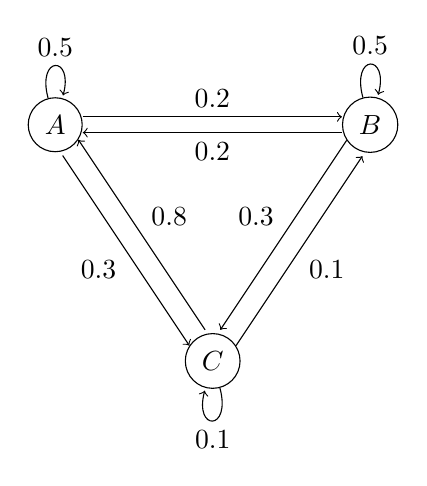
\begin{tikzpicture}
    \node[shape=circle,draw=black] (1) at (0,0) {$A$};
    \node[shape=circle,draw=black] (2) at (4,0) {$B$};
    \node[shape=circle,draw=black] (3) at (2,-3) {$C$};

    \path [->] (1)
            edge [loop above] node
            {$0.5$} (1);
    \path [transform canvas={yshift=0.1cm},->] (1)
            edge [above] node
            {$0.2$} (2);
    \path [transform canvas={xshift=-0.1cm,yshift=-0.1cm},->] (1)
            edge [below left] node
            {$0.3$} (3);
    \path [->] (2)
            edge [loop above] node
            {$0.5$} (2);
    \path [transform canvas={yshift=-0.1cm},->] (2)
            edge [below] node
            {$0.2$} (1);
    \path [transform canvas={xshift=-0.1cm,yshift=0.1cm},->] (2)
            edge [above left] node
            {$0.3$} (3);
    \path [->] (3)
            edge [loop below] node
            {$0.1$} (3);
    \path [transform canvas={xshift=0.1cm,yshift=-0.1cm},->] (3)
            edge [below right] node
            {$0.1$} (2);
    \path [transform canvas={xshift=0.1cm,yshift=0.1cm},->] (3)
            edge [above right] node
            {$0.8$} (1);
\end{tikzpicture}
\end{center}

\begin{flushleft}
Der Prozess kann mit der Übergangsmatrix $P$ beschrieben werden:
\begin{align}
    P=\begin{pmatrix}
        0.5 & 0.2 & 0.8 \\
        0.2 & 0.5 & 0.1 \\
        0.3 & 0.3 & 0.1
    \end{pmatrix}
\end{align}

Hierbei ist wichtig zu beachten, dass die Ausrichtung der Matrix anders ist als bei ein- und zweistufigen Prozessen.

Ausrichtung bei $P$:
\end{flushleft}

\begin{center}
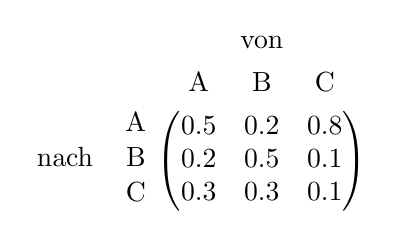
\begin{tikzpicture}
    \node (P) at (0,0)
        {$\begin{pmatrix}
            0.5 & 0.2 & 0.8 \\
            0.2 & 0.5 & 0.1 \\
            0.3 & 0.3 & 0.1
        \end{pmatrix}$};
    \node (2) at (0,1.5) {von};
    \node (A1) at (-0.8,1) {A};
    \node (B1) at (0,1) {B};
    \node (C1) at (0.8,1) {C};
    \node (3) at (-2.5,0.05) {nach};
    \node (A2) at (-1.6,-0.4) {C};
    \node (B2) at (-1.6,0.05) {B};
    \node (C2) at (-1.6,0.5) {A};
\end{tikzpicture}
\end{center}

\begin{flushleft}  
Ausrichtung bei $A$ vom Beispiel aus Kapitel \ref{subsec:2proc}:
\end{flushleft}

\begin{center}
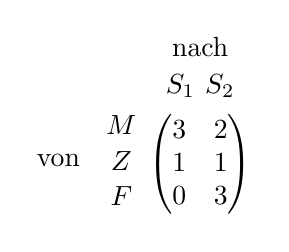
\begin{tikzpicture}
    \node (P) at (0,0)
        {$\begin{pmatrix}
            3 & 2 \\
            1 & 1 \\
            0 & 3
        \end{pmatrix}$};
    \node (2) at (0,1.5) {nach};
    \node (A1) at (-0.25,1) {$S_1$};
    \node (B1) at (0.25,1) {$S_2$};
    \node (3) at (-1.8,0.05) {von};
    \node (A2) at (-1,-0.4) {$F$};
    \node (B2) at (-1,0.05) {$Z$};
    \node (C2) at (-1,0.5) {$M$};
\end{tikzpicture}
\end{center}

\begin{flushleft}
So lässt sich relativ leicht berechnen, wie viele Tiere am nächsten Tag an den Tränken sind, wenn am vorherigen Tag $x_1=1000$ bei $A$, $x_2=1000$ bei $B$ und $x_3=400$ bei $C$ sind:
\begin{align}
    P&\cdot\vec{x} \\
    \begin{pmatrix}
        0.5 & 0.2 & 0.8 \\
        0.2 & 0.5 & 0.1 \\
        0.3 & 0.3 & 0.1
    \end{pmatrix}\cdot
    \begin{pmatrix}
        1000 \\
        1000 \\
        400
    \end{pmatrix}&=
    \begin{pmatrix}
        1020 \\
        740 \\
        640
    \end{pmatrix}
\end{align}

Bei diesem Prozess ist die Spaltensumme der Übergangsmatrix immer $1$, daher verändert sich die Gesamtanzahl der Tiere nicht.
\begin{align}
    0.5+0.2+0.3=1 \\
    0.2+0.5+0.3=1 \\
    0.8+0.1+0.1=1
\end{align}

Da die Elemente von $P$ auch als Wahrscheinlichkeiten interpretiert werden können, ist $P$ eine stochastische Matrix.

Eine Matrix $A$ gilt als stochastisch, wenn:
\begin{itemize}
    \item {
        sie quadratisch ist,
    }
    \item {
        für jedes ihrer Elemente $a_{ij}$, $a_{ij} \in [0,1]$ gilt und
    }
    \item {
        die Summe der Elemente in jeder Spalte $1$ ist.
    }
\end{itemize}

Besonders interessant an Austauschprozessen ist die langfristige Entwicklung.
Verwendet man immer dieselbe Matrix $P$, spricht man von einer Markoff'schen Kette.
\end{flushleft}

\begin{center}
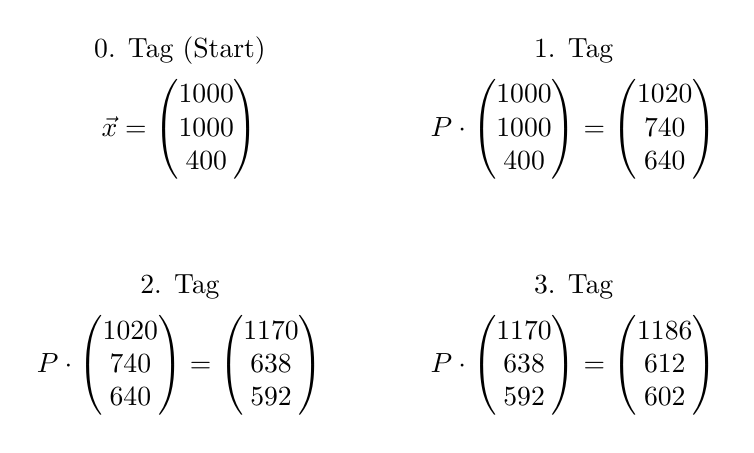
\begin{tikzpicture}
    \node (0) at (0,1)
            {0. Tag (Start)};
    \node (p0) at (0,0)
            {$\vec{x}=\begin{pmatrix} 1000 \\ 1000 \\ 400 \end{pmatrix}$};
    \node (1) at (5,1)
            {1. Tag};
    \node (p1) at (5,0)
            {$P\cdot\begin{pmatrix}
                1000 \\
                1000 \\
                400
            \end{pmatrix}=
            \begin{pmatrix}
                1020 \\
                740 \\
                640
            \end{pmatrix}$};
    \node (2) at (0,-2)
            {2. Tag};
    \node (p2) at (0,-3)
            {$P\cdot\begin{pmatrix}
                1020 \\
                740 \\
                640
            \end{pmatrix}=
            \begin{pmatrix}
                1170 \\
                638 \\
                592
            \end{pmatrix}$};
    \node (3) at (5,-2)
            {3. Tag};
    \node (p3) at (5,-3)
            {$P\cdot\begin{pmatrix}
                1170 \\
                638 \\
                592
            \end{pmatrix}=
            \begin{pmatrix}
                1186 \\
                612 \\
                602
            \end{pmatrix}$};
\end{tikzpicture}
\end{center}

\begin{flushleft}
Anstatt die Verteilung am 3. Tag schrittweise zu berechnen, kann die Verteilung auch direkt mit $P^3\cdot\vec{x}$ berechnet werden.
Für die Verteilung $\vec{v}_n$ am $n$-ten Tag gilt also:
\begin{align}
    \vec{v}_n=P^n\cdot\vec{x}
\end{align}

Die Verteilung strebt eine stabile Verteilung $\vec{g}=\begin{pmatrix} 1200 \\ 600 \\ 600 \end{pmatrix}$ an, die auch Gleichgewichtsverteilung genannt wird.

Zu der Matrix $P$ gehört eine Grenzmatrix $G$:
\begin{align}
    G&=\lim_{k\to\infty} P^k \\
    G&=\begin{pmatrix}
        0.5 & 0.5 & 0.5 \\
        0.25 & 0.25 & 0.25 \\
        0.25 & 0.25 & 0.25
    \end{pmatrix}
\end{align}

Außerdem kann ein Fixvektor $\vec{g}$ zu $P$ bestimmt werden:
\begin{align}
    P\cdot\vec{g}&=\vec{g} \\
    P\cdot\begin{pmatrix} g_1 \\ g_2 \\ g_3 \end{pmatrix}&=\begin{pmatrix} g_1 \\ g_2 \\ g_3 \end{pmatrix}
\end{align}

Es gibt unendlich viele Lösungen, da $g_1=2g_3$ und $g_2=g_3$.

Für $g_3=t$ gilt also:
\begin{align}
    \vec{g}_t=t\cdot\begin{pmatrix} 2 \\ 1 \\ 1 \end{pmatrix}
\end{align}

Der vorherige Startvektor $\vec{x}=\begin{pmatrix} 1000 \\ 1000 \\ 400 \end{pmatrix}$ hat eine Gesamtanzahl an Tieren von 2400.
Es gilt also $x_1+x_2+x_3=2400$.
Um $t$ für diesen Vektor herauszufinden gilt es also $2t+t+t=2400$ zu lösen:
\begin{align}
    2t+t+t&=2400 \\
    \Leftrightarrow\quad 4t&=2400 \\
    \Leftrightarrow\quad t&=600
\end{align}

Der Fixvektor $\vec{g}_{600}$ ist also:
\begin{align}
    \vec{g}&=600\cdot\begin{pmatrix} 2 \\ 1 \\ 1 \end{pmatrix} \\
    \vec{g}&=\begin{pmatrix} 1200 \\ 600 \\ 600 \end{pmatrix}
\end{align}
\end{flushleft}

\subsection{Populationsentwicklungen}
\begin{flushleft}
Populationsentwicklungen sind ähnlich zu Austauschprozessen.
Die Übergangsmatrix ist jedoch keine stochastische Matrix, demnach sind die Spaltensummen nicht $1$.

Hier ein Beispiel bei dem monatlich $25\%$ der Eier $E$ zu Larven $L$ wachsen,
von diesen Larven $L$ wachsen monatlich $50\%$ zu Insekten $I$,
jedes Insekt $I$ legt monatlich acht Eier $E$:
\end{flushleft}

\begin{center}
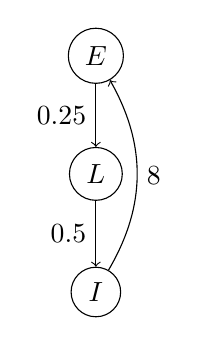
\begin{tikzpicture}
    \node[shape=circle,draw=black] (E) at (0,0) {$E$};
    \node[shape=circle,draw=black] (L) at (0,-1.5) {$L$};
    \node[shape=circle,draw=black] (I) at (0,-3) {$I$};

    \path [->] (E) edge [left] node {$0.25$} (L);
    \path [->] (L) edge [left] node {$0.5$} (I);
    \path [->] (I) edge [bend right,right] node {$8$} (E);
\end{tikzpicture}
\end{center}

\begin{center}
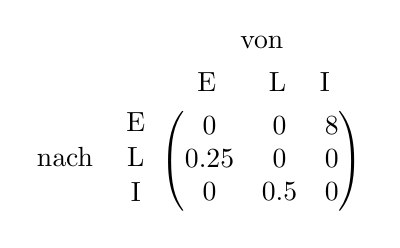
\begin{tikzpicture}
    \node (A) at (0,0)
        {$\begin{pmatrix}
            0    & 0   & 8 \\
            0.25 & 0   & 0 \\
            0    & 0.5 & 0
        \end{pmatrix}$};
    \node (2) at (0,1.5) {von};
    \node (A1) at (-0.7,1) {E};
    \node (B1) at (0.2,1) {L};
    \node (C1) at (0.8,1) {I};
    \node (3) at (-2.5,0.05) {nach};
    \node (A2) at (-1.6,-0.4) {I};
    \node (B2) at (-1.6,0.05) {L};
    \node (C2) at (-1.6,0.5) {E};
\end{tikzpicture}
\end{center}

\begin{flushleft}
Die Übergangsmatrix $A$ des Modells ist also:
\begin{align}
    A=\begin{pmatrix}
        0    & 0   & 8 \\
        0.25 & 0   & 0 \\
        0    & 0.5 & 0
    \end{pmatrix}
\end{align}

Die Startpopulation in diesem Modell wird mit $\vec{p}_1$ dargestellt:
\begin{align}
    \vec{p}_1=\begin{pmatrix} 120 \\ 40 \\ 24 \end{pmatrix}
\end{align}

Demnach beträgt die Population zum Anfang des 2. Monats:
\begin{align}
    \vec{p}_2=A\cdot\begin{pmatrix}
        120 \\ 40 \\ 24
    \end{pmatrix}=\begin{pmatrix}
        192 \\ 30 \\ 20
    \end{pmatrix}
\end{align}
\end{flushleft}

\begin{center}
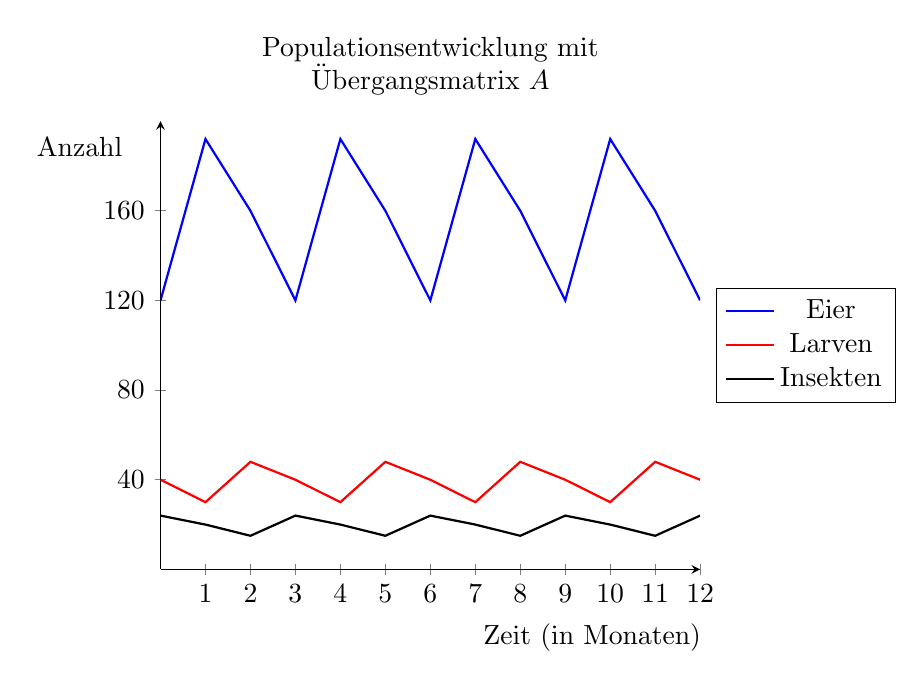
\begin{tikzpicture}
\begin{axis}[
    axis lines=center,
    title={Populationsentwicklung mit \\ Übergangsmatrix $A$},
    title style={align=center},
    xlabel={Zeit (in Monaten)},
    ylabel={Anzahl},
    x label style={at={(axis description cs:0.8,-0.1)},anchor=north},
    y label style={at={(axis description cs:-0.15,0.9)},anchor=south},
    xmin=0,xmax=12,
    ymin=0,ymax=200,
    xtick={0,1,2,3,4,5,6,7,8,9,10,11,12},
    ytick={0,40,80,120,160},
    legend style={
        at={(1.03,0.5)},
        anchor=west
    }
]

\addplot[color=blue,thick] coordinates {
    (0,120) (1,192) (2,160)
    (3,120) (4,192) (5,160)
    (6,120) (7,192) (8,160)
    (9,120) (10,192) (11,160)
    (12,120)
};
\addlegendentry{Eier}

\addplot[color=red,thick] coordinates {
    (0,40) (1,30) (2,48)
    (3,40) (4,30) (5,48)
    (6,40) (7,30) (8,48)
    (9,40) (10,30) (11,48)
    (12,40)
};
\addlegendentry{Larven}

\addplot[color=black,thick] coordinates {
    (0,24) (1,20) (2,15)
    (3,24) (4,20) (5,15)
    (6,24) (7,20) (8,15)
    (9,24) (10,20) (11,15)
    (12,24)
};
\addlegendentry{Insekten}

\end{axis}
\end{tikzpicture}
\end{center}

\begin{flushleft}
An dem Graphen sieht man relativ gut, dass sich die Populationen zyklisch entwickeln.

Eine quadratische Matrix $A$ ist zyklisch, wenn ein $n\in\mathbb{N}$ existiert, für das $A^n=E$ gilt.
In diesem Beispiel gilt das für $n=3$:
\begin{align}
    \vec{p}_4=A^3\cdot\begin{pmatrix}
        120 \\ 40 \\ 24
    \end{pmatrix}=
    \begin{pmatrix}
        120 \\ 40 \\ 24
    \end{pmatrix}
\end{align}

Die Entwicklung verläuft anders, wenn ein Insekt nur noch vier Eier legen kann.
Diese Situation wird durch die Übergangsmatrix $B$ modelliert:
\begin{align}
    B=\begin{pmatrix}
        0    & 0   & 4 \\
        0.25 & 0   & 0 \\
        0    & 0.5 & 0
    \end{pmatrix}
\end{align}
\end{flushleft}

\begin{center}
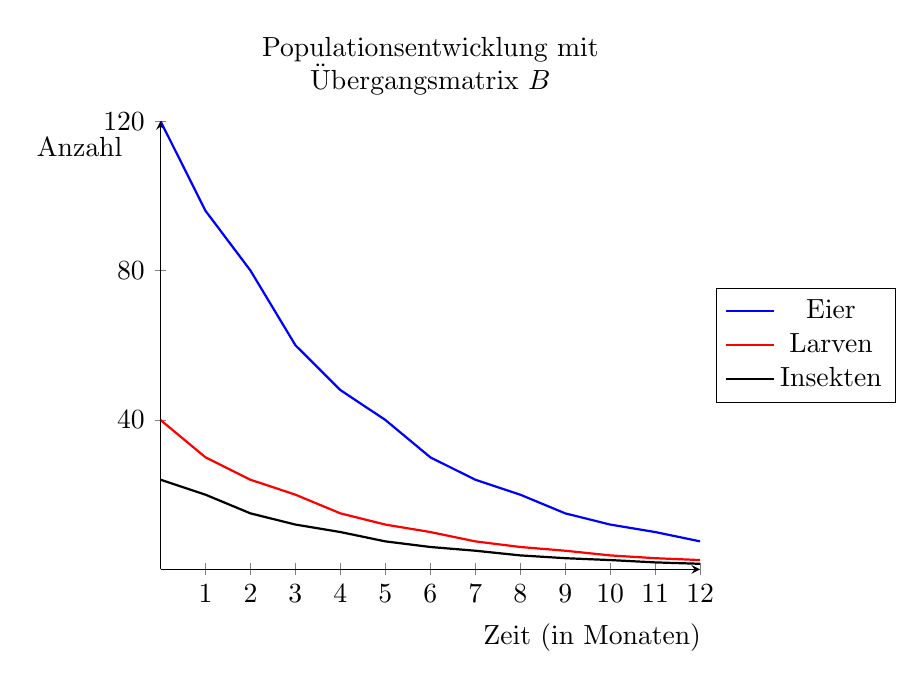
\begin{tikzpicture}
\begin{axis}[
    axis lines=center,
    title={Populationsentwicklung mit \\ Übergangsmatrix $B$},
    title style={align=center},
    xlabel={Zeit (in Monaten)},
    ylabel={Anzahl},
    x label style={at={(axis description cs:0.8,-0.1)},anchor=north},
    y label style={at={(axis description cs:-0.15,0.9)},anchor=south},
    xmin=0,xmax=12,
    ymin=0,ymax=120,
    xtick={0,1,2,3,4,5,6,7,8,9,10,11,12},
    ytick={0,40,80,120},
    legend style={
        at={(1.03,0.5)},
        anchor=west
    }
]

\addplot[color=blue,thick] coordinates {
    (0,120) (1,96) (2,80)
    (3,60) (4,48) (5,40)
    (6,30) (7,24) (8,20)
    (9,15) (10,12) (11,10)
    (12,7.5)
};
\addlegendentry{Eier}

\addplot[color=red,thick] coordinates {
    (0,40) (1,30) (2,24)
    (3,20) (4,15) (5,12)
    (6,10) (7,7.5) (8,6)
    (9,5) (10,3.75) (11,3)
    (12,2.5)
};
\addlegendentry{Larven}

\addplot[color=black,thick] coordinates {
    (0,24) (1,20) (2,15)
    (3,12) (4,10) (5,7.5)
    (6,6) (7,5) (8,3.75)
    (9,3) (10,2.5) (11,1.875)
    (12,1.5)
};
\addlegendentry{Insekten}

\end{axis}
\end{tikzpicture}
\end{center}

\begin{flushleft}
Mit $B$ als Übergangsmatrix halbiert sich die Population innerhalb von drei Monaten,
da:
\begin{align}
    B&=\begin{pmatrix}
        0    & 0   & 4 \\
        0.25 & 0   & 0 \\
        0    & 0.5 & 0
    \end{pmatrix} \\
    B^3&=\begin{pmatrix}
        0.5 & 0   & 0 \\
        0   & 0.5 & 0 \\
        0   & 0   & 0.5
    \end{pmatrix} \\
    B^6&=\begin{pmatrix}
        0.25 & 0   & 0 \\
        0    & 0.25 & 0 \\
        0    & 0    & 0.25
    \end{pmatrix}
\end{align}

Allgemein gilt für Prozesse dieser Art die Übergangsmatrix 
$
U=\begin{pmatrix}
    0 & 0 & v \\
    a & 0 & 0 \\
    0 & b & 0
\end{pmatrix}
$
, $v$ steht für die Vermehrungsrate, $a$ und $b$ jeweils für die Überlebensraten.

Die Übergangsmatrix $U$ kann nur einer Population zugeordnet werden, wenn $v>0$ ist und $a,b\in]0,1]$ sind.

Besonders relevant ist $U^3$:
\begin{align}   
    U^3=\begin{pmatrix}
        a\cdot b\cdot v & 0 & 0 \\
        0 & a\cdot b\cdot v & 0 \\
        0 & 0 & a\cdot b\cdot v
    \end{pmatrix}
\end{align}

Hieraus lässt sich schließen, dass folgendes gilt:
\[
    \text{Wenn}
\begin{cases}
    a\cdot b\cdot v < 1,& \text{ist, stribt die Population aus.} \\
    a\cdot b\cdot v = 1,& \text{ist, entwickelt sich die Population zyklisch.} \\
    a\cdot b\cdot v > 1,& \text{ist, wächst die Population.}
\end{cases}
\]

Dieses Verhalten lässt sich auch gut an den Übergangsmatrizen $A$ und $B$ erkennen.

Für $A$ gilt:
\begin{align}
    a\cdot b\cdot v&=0.25\cdot 0.5\cdot 8=1 \\
    A^3&=1\cdot E=E
\end{align}

Für $B$ gilt:
\begin{align}
    a\cdot b\cdot v&=0.25\cdot 0.5\cdot 4=0.5 \\
    B^3&=0.5\cdot E
\end{align}

Demnach entwickelt sich die Population, die durch $A$ beschrieben wird zyklisch
und die durch $B$ beschriebene Population stirbt aus.
\end{flushleft}

\subsection{Affine Abbildungen}
\subsubsection{Verschiebung}
\begin{center}
\begin{tikzpicture}
\begin{axis}[
    axis lines=center,
    title={Die Verschiebung des Punktes $P(1,1)$ zum Punkt $P'(3,1)$},
    title style={align=center},
    xlabel={$x_1$},
    ylabel={$x_2$},
    xmin=0,xmax=4,
    ymin=0,ymax=2
]

\addplot[mark=*] coordinates {(1,1)} node[label={90:{$P$}}]{};
\addplot[mark=*] coordinates {(3,1)} node[label={90:{$P'$}}]{};

\end{axis}
\end{tikzpicture}
\end{center}

\begin{flushleft}
Diese Verschiebung kann durch diese Gleichungen dargestellt werden:
\begin{align}
    x_1'=x_1+2 \\
    x_2'=x_2+0
\end{align}

Die Gleichungen lassen sich auch durch Vektoren darstellen:
\begin{align}
    \begin{pmatrix}
        x_1' \\
        x_2'
    \end{pmatrix}=\begin{pmatrix}
        x_1 \\
        x_2
    \end{pmatrix}+\begin{pmatrix}
        2 \\
        0
    \end{pmatrix}
\end{align}

Allgemein gilt also:
\begin{align}
    \begin{pmatrix}
        x_1' \\
        x_2'
    \end{pmatrix}=\begin{pmatrix}
        x_1 \\
        x_2
    \end{pmatrix}+\vec{c}
\end{align}

oder:
\begin{align}
    \alpha\colon \vec{x'}=\vec{x}+\vec{c}
\end{align}

für eine Abbildung $\alpha$, die eine Verschiebung darstellt.
\end{flushleft}

\subsubsection{Skalierung}
\begin{center}
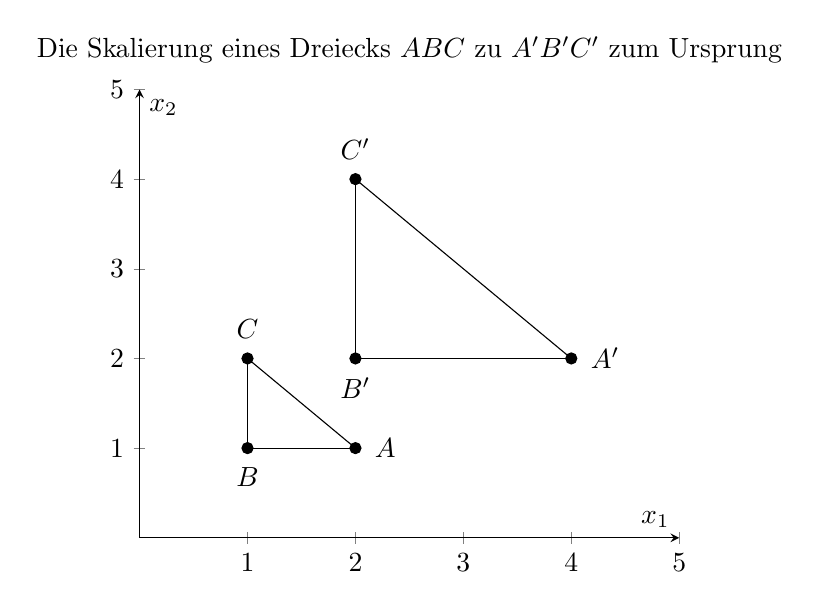
\begin{tikzpicture}
\begin{axis}[
    axis lines=center,
    title={Die Skalierung eines Dreiecks $ABC$ zu $A'B'C'$ zum Ursprung},
    title style={align=center},
    xlabel={$x_1$},
    ylabel={$x_2$},
    xmin=0,xmax=5,
    ymin=0,ymax=5
]

\addplot[mark=*] coordinates {(2,1)} node[label={0:{$A$}}]{};
\addplot[mark=*] coordinates {(1,1)} node[label={270:{$B$}}]{};
\addplot[mark=*] coordinates {(1,2)} node[label={90:{$C$}}]{};
\draw (axis cs:1,1) -- (axis cs:2,1);
\draw (axis cs:1,1) -- (axis cs:1,2);
\draw (axis cs:2,1) -- (axis cs:1,2);

\addplot[mark=*] coordinates {(4,2)} node[label={0:{$A'$}}]{};
\addplot[mark=*] coordinates {(2,2)} node[label={270:{$B'$}}]{};
\addplot[mark=*] coordinates {(2,4)} node[label={90:{$C'$}}]{};
\draw (axis cs:2,2) -- (axis cs:4,2);
\draw (axis cs:2,2) -- (axis cs:2,4);
\draw (axis cs:4,2) -- (axis cs:2,4);

\end{axis}
\end{tikzpicture}
\end{center}

\begin{flushleft}
Diese Skalierung zum Ursprung kann durch diese Gleichungen dargestellt werden:
\begin{align}
    x_1'=2x_1 \\
    x_2'=2x_2
\end{align}

Die Gleichungen lassen sich auch durch Vektoren darstellen:
\begin{align}
    \begin{pmatrix}
        x_1' \\
        x_2'
    \end{pmatrix}=2\begin{pmatrix}
        x_1 \\
        x_2
    \end{pmatrix}
\end{align}

Allgemein gilt also:
\begin{align}
    \begin{pmatrix}
        x_1' \\
        x_2'
    \end{pmatrix}=r\begin{pmatrix}
        x_1 \\
        x_2
    \end{pmatrix}
\end{align}

oder:
\begin{align}
    \alpha\colon \vec{x'}=r\vec{x}
\end{align}

für eine Abbildung $\alpha$, die eine Skalierung zum Ursprung darstellt.
\end{flushleft}

\chapter{Weitere Regeln}

\section{Potenzgesetze}
\begin{align}
    a^0 &= 1 \\
    \frac{1}{a^n} &= a^{-n} \\
    a^n*a^m &= a^{n+m} \\
    \frac{a^n}{a^m} &= a^{n-m} \\
    a^n*b^n &= (a*b)^n \\
    \frac{a^n}{b^n} &= \left(\frac{a}{b}\right)^n \\
    \left(a^n\right)^m &= a^{n*m} \\
    a^{\frac{m}{n}} &= \sqrt[n]{a^m}=\left(\sqrt[n]{a}\right)^m
\end{align}

\section{Ableitungsregeln}
\begin{align}
    \left(x^n\right)' &=n*x^{n-1} \\
    \left(a*x^n\right)' &=a*n*x^{n-1} \\
    \left[f(x)+g(x)\right]' &=f'(x)+g'(x)
\end{align}

\section{Sigma-Umgebungen}
\begin{align}
    \sigma \approx 68.3\% \\
    2\sigma \approx 95.4\% \\
    3\sigma \approx 99.7\% \\
    1.64\sigma \approx 90\% \\
    1.96\sigma \approx 95\% \\
    2.58\sigma \approx 99\%
\end{align}

\end{document}
